% Chapter 9

\chapter{Analysis of 2016 raw multiplicities} % Chapter title

\label{ch:raw} % For referencing the chapter elsewhere, use \autoref{ch:name}

The 2006 SIDIS COMPASS hadron multiplicity results, based on data taken with an isoscalar target ($^6$LiD), do not constrain fermly the strange quark fragmentation function.
With the analysis of new data taken on pure proton target (lH$_2$), the results will provide a new set of equations linking the multiplicities with the fragmentation functions but still involving the same quark fragmentation functions we are interested in. The fact that the proton and deuteron data can be fitted together will add constrains to the fragmentation function extraction.
In order to perform this kind of study, one need a precision of 5 to 7\% on the multiplicities.

The analysis is performed on COMPASS data recorded in 2016 using a 160 GeV muon beam incident on a proton target (lH$_2$). Five weeks of the 2016 data are analyzed (named P07, P08, P09, P10 and P11).

%----------------------------------------------------------------------------------------

\section{Method of extraction}

The method of extraction of the multiplicities follow several steps. For each selection step,
a list of cuts is applied on both geometrical and physical quantities. First the DIS events are selected
and then the SIDIS events (hadrons) are selected. For the DIS event selection, a study on the target radius had to be made in order to determine the optimal value for the target cut. When the event selection is done, the hadrons have to be identified between pions, kaons and protons and the identification has to be corrected according to the RICH detection efficiency and purity in a process called unfolding. The obtained raw multiplicities are then binned. The general event reconstruction codes for COMPASS are used. A personal analysis code is developed to study the SIDIS channel and select pion, kaon or protons production events.

In the following, the effect of the cuts for both DIS events and hadron selection is summarized in a table, showing the number of DIS events and hadrons and the absolute percentage of the sample remaining. When the numbers are not specified, it is because the recovery of the number is too complex due to the transversal implementation of the cut in the code (e.g. for the $\nu$ cut).

In a pre-analysis, the whole sample has been pre-filtered into so-called $\mu$DSTs asking for at least one primary vertex (PV) with well measured beam momentum, for at least one outgoing $\mu$ with the same charge of the incoming one and for $Q^2$ $>$ 0.8 (GeV/$c$)$^2$. Another pre-analysis selects also the Best Primary Vertices and whether there is a reconstructed scattered muon. It explains why in the cut flow for the selection of DIS events, there is no effect for these two cuts.

%------------------------------------------------

\section{DIS event selection}

For the DIS event selection ($\mu p \rightarrow \mu X$), the following list of cuts is applied :

\newpage

\begin{table}[!h]
  \centering
  \begin{tabular}{p{10cm} p{2cm} p{2cm}}
    \hline
    \hline
     Cut & \# of events after cut & Absolute \% of events after cut  \\
    \hline
    \hline
    Events with Best Primary Vertex & 47.5 M & 100\% \\
    Events with reconstruted scattered muon & 47.5 M & 100\% \\
    Events with primary interaction in the target material, target radius cut (explained in Section \ref{sec:targetcut}) & 25.6 M & 53.8\% \\
    Events with energy of beam muon energy in range [140 GeV, 180 GeV] & 25.6 M & 53.8\% \\
    Events with a well reconstructed beam track (so-called 'BMS cut') & 24.2 M & 50.9\% \\
    Events with $\chi^2$/ndf $<$ 10 for a well reconstructed beam track & 24.2 M & 50.9\% \\
    Events with muon beam trajectory crossing entirely the target cell & 23.4 M & 49.2\% \\
    Events with $\chi^2$/ndf $<$ 10 for a well reconstructed scattered muon track & 23.4 M & 49.2\% \\
    Events with Z coordinate of the first measured hit of scattered muon $<$ 350 cm ($Z_{SM1}$) & 23.3 M & 49.1\% \\
    Events with Middle, Ladder, Outer or LAST trigger & 23.3 M & 49.1\% \\
    Events with $Q^2>1$ (GeV/$c$)$^2$ & 18.5 M & 38.9\% \\
    Events with $0.1 < y < 0.7$ & 8.39 M & 17.7\% \\
    Events with $5 < W < 17$ GeV/$c^2$ & 8.34 M & 17.6\% \\
    Events with $0.004 < x < 0.4$ & 8.32 M & 17.5\% \\
    Events with $\nu$ cut & - & - \\
    \hline
    \hline
  \end{tabular}
\end{table}

The cut $Q^2>1$ (GeV/$c$)$^2$ is to be in the deep inelastic scattering regime. The lower limit $W > 5$ GeV/$c^2$ is to avoid the region of target fragmentation and the upper limit $W < 17$ GeV/$c^2$ to avoid low statistic region. Concerning the $y$ cut, the lower limit $y > 0.1$ removes events with bad reconstruction of scattered muon (momentum resolution deterioration at low angle) and the misidentification of halo muons as scattered muons. The upper limit $y < 0.7$ eliminates events where large radiative corrections are applied (corrections greater than 20\%).

Concerning the triggers, four triggers are used in this analysis : the middle trigger (MT), the ladder trigger (LT), the outer trigger (OT) and the las trigger (LAST). They are all inclusive triggers, ie. only a scattered $\mu$ is required to fire the triggers. The region covered by triggers as a function of $x$ and $Q^2$ is shown in Fig. \ref{pic:triggerxQ2}. The middle trigger covers the low $Q^2$ region, the ladder trigger covers the middle $Q^2$ region while the outer and las cover the high $Q^2$ region. For $x$, the outer covers the low and high $x$, while middle and ladder cover the middle $x$ region and the las the high $x$ region.

In 2016, central slabs of the outer trigger were cured from their inefficiency from P08 onward. Thus it was decided to keep them cut out for P07 by geometrical cut and incorporate them for P08 and following periods. The events in P07 where the scattered $\mu$ track goes through the inefficient slabs are rejected.

\begin{figure}[!h]
	% 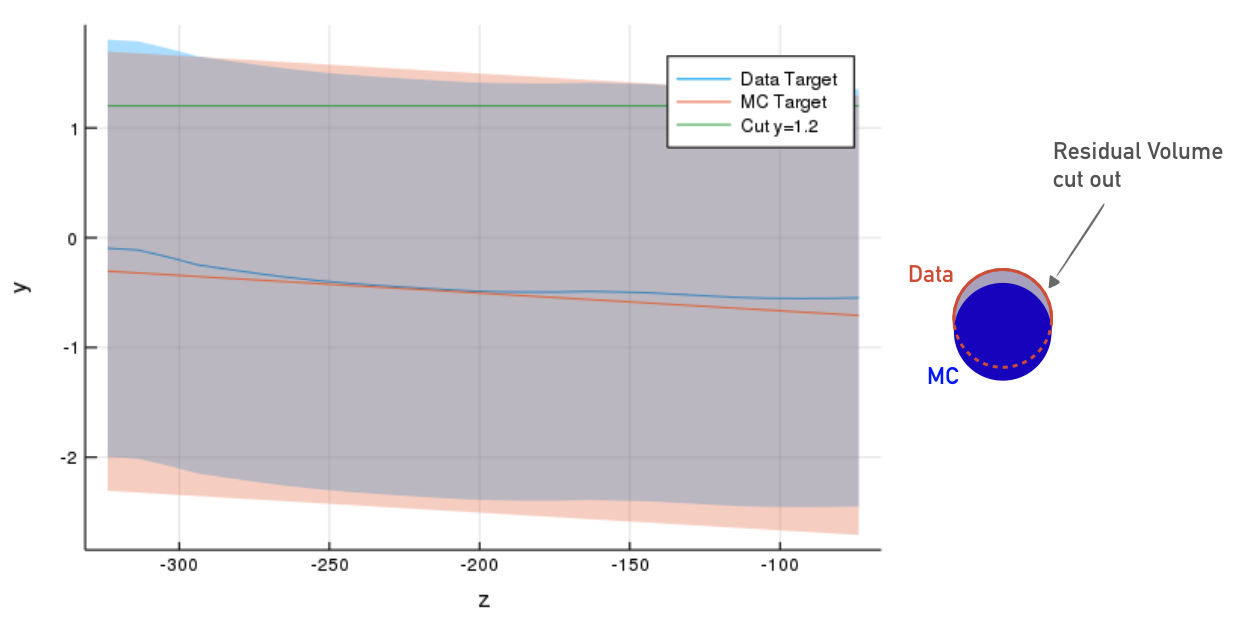
\includegraphics[scale=0.4]{./gfx/Targetcut.png}
	\caption{Event distribution for the middle, ladder, outer and las triggers as a function of $Q^2$ (a) and $x$ (b).}
	\label{pic:triggerxQ2}
\end{figure}

The cut on the kinematic variable $\nu$ was implemented to reject events that contain hadrons outside of the measured
momentum range of 12 - 40 GeV/c. The criteria is defined by :
\begin{equation}
  \nu_{max} = \frac{\sqrt{(p^2_{max}+m^2_h)}}{z_{max}}
\end{equation}
\begin{equation}
  \nu_{min} = \frac{\sqrt{(p^2_{min}+m^2_h)}}{z_{min}}
\end{equation}

where $p_{max}$ (resp. $p_{min}$) is the hadron momentum limit of 40 GeV/c (resp. 12 GeV/c), $z_{max}$ (resp. $z_{min}$)
is the upper (resp. lower) value of the $z$-bin and $m_h$ is the mass of the considered hadron.

The $Q^2$, $x$ and $y$ distributions are illustrated in Fig. \ref{pic:DISdist} for the DIS sample after event selections. The $Q^2$-$x$ correlation is also shown as well as the $x$-$y$ one. It can be noted that most of the statistics is located in the low $Q^2$-$x$ and low $x$-$y$ values and $Q^2$ values reach up to 90 (GeV/$c$)$^2$.

\begin{figure}[!h]
  \subfloat[$Q^2$]{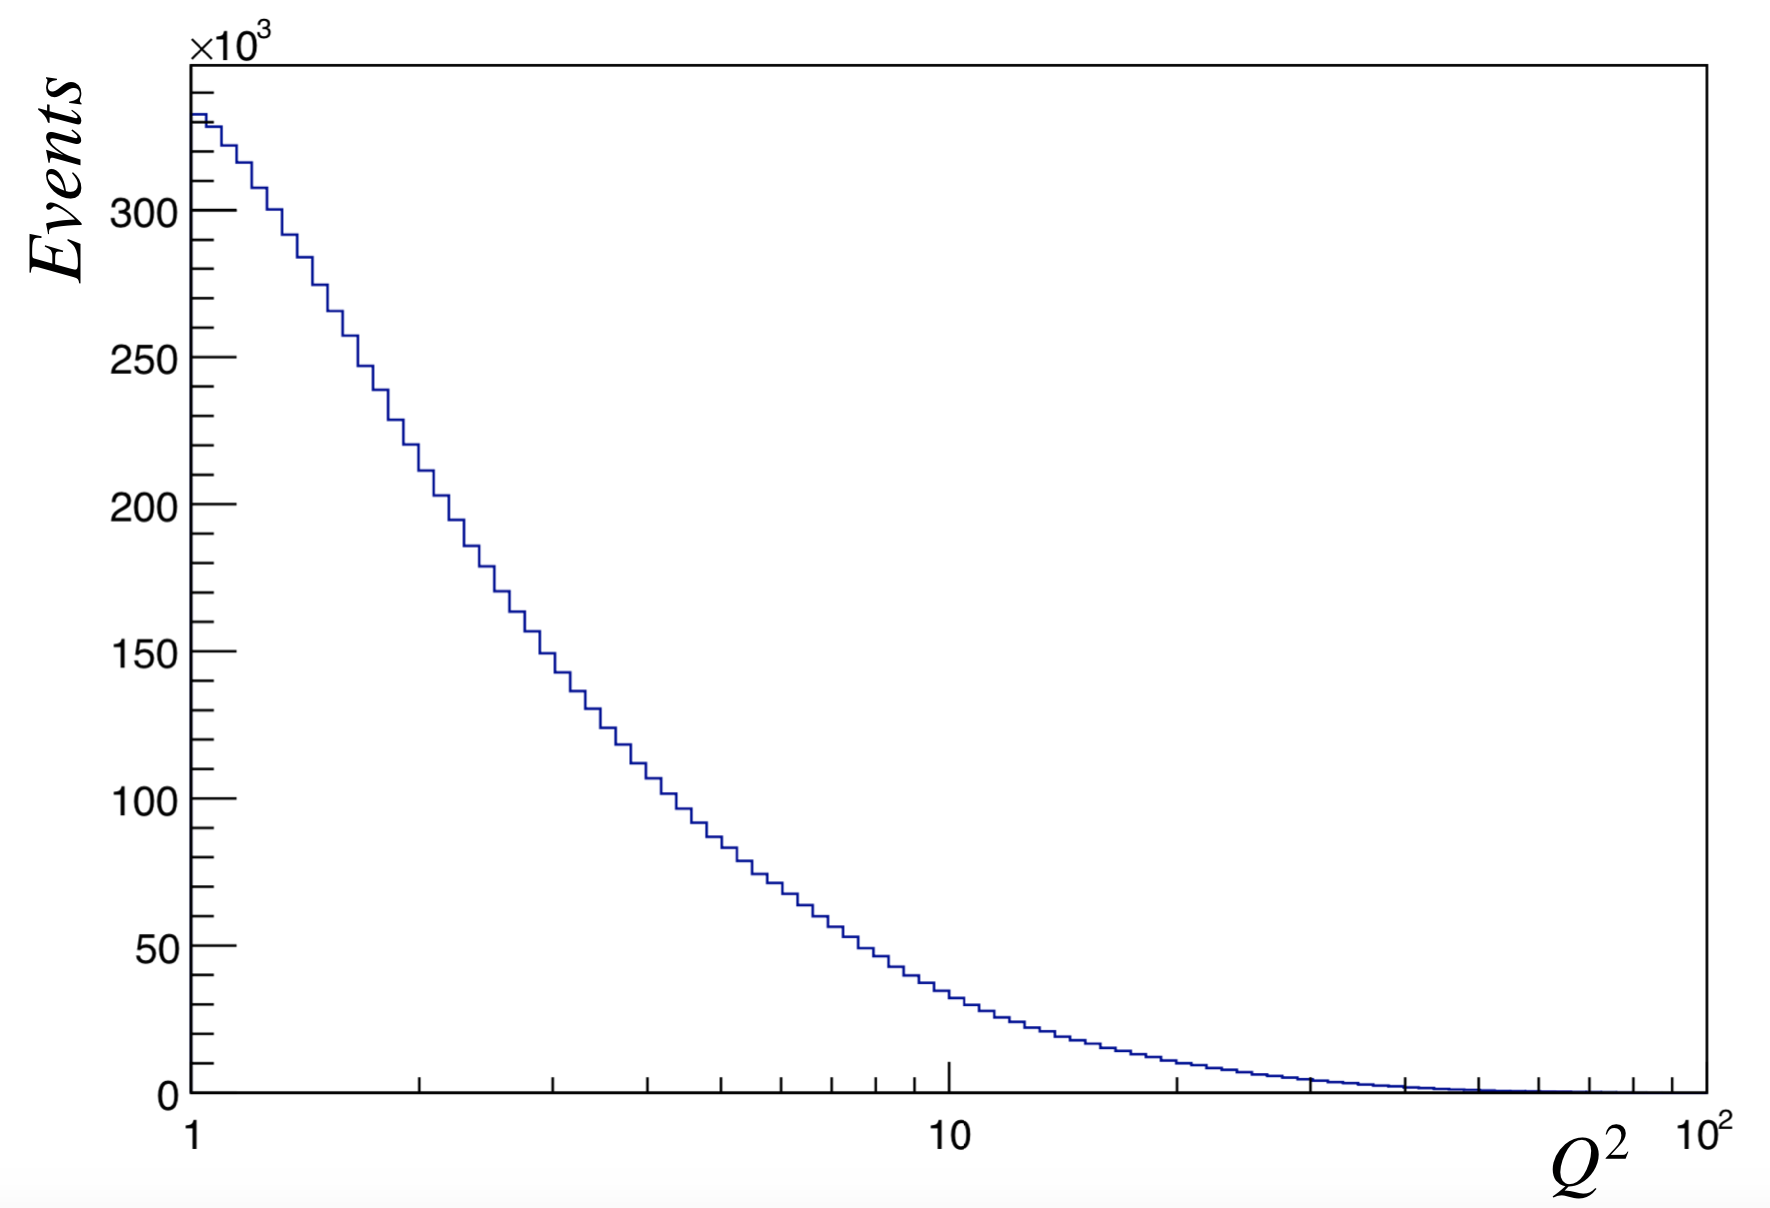
\includegraphics[scale=0.27]{./gfx/Q2DIS.png}}
  \subfloat[$x$]{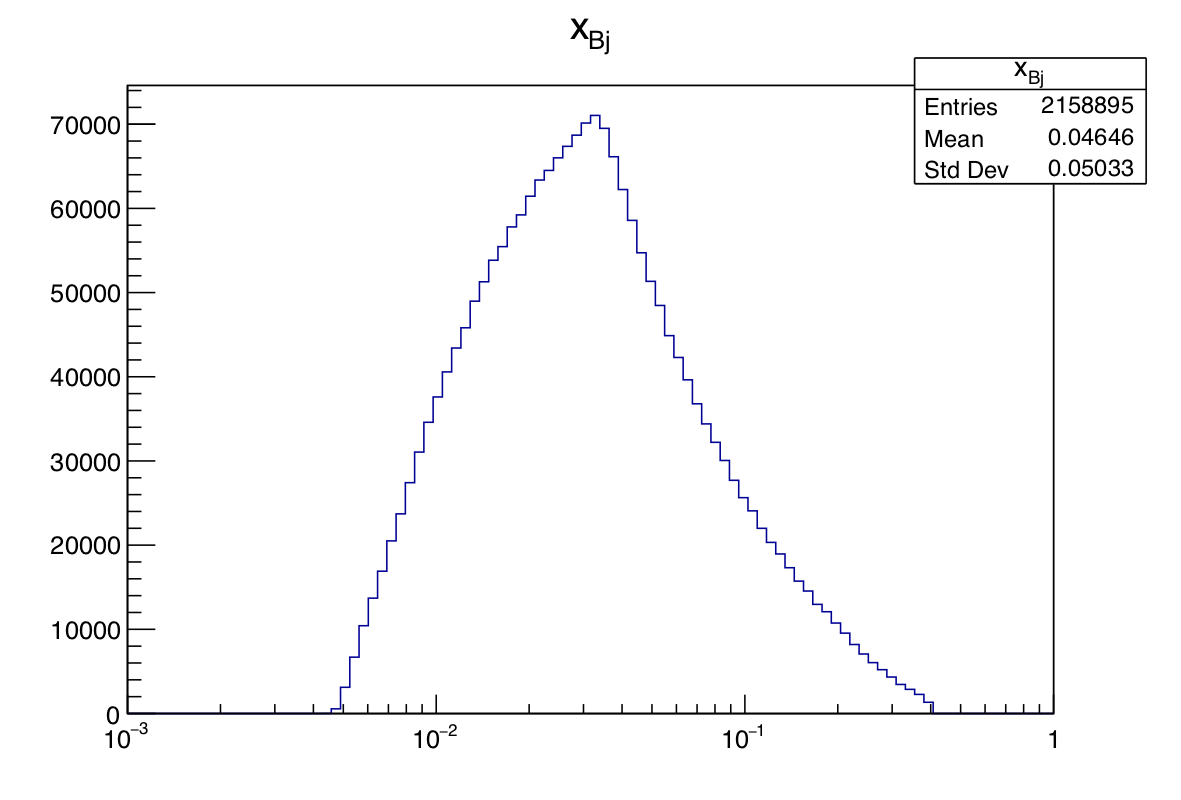
\includegraphics[scale=0.27]{./gfx/xDIS.png}}
  \subfloat[$y$]{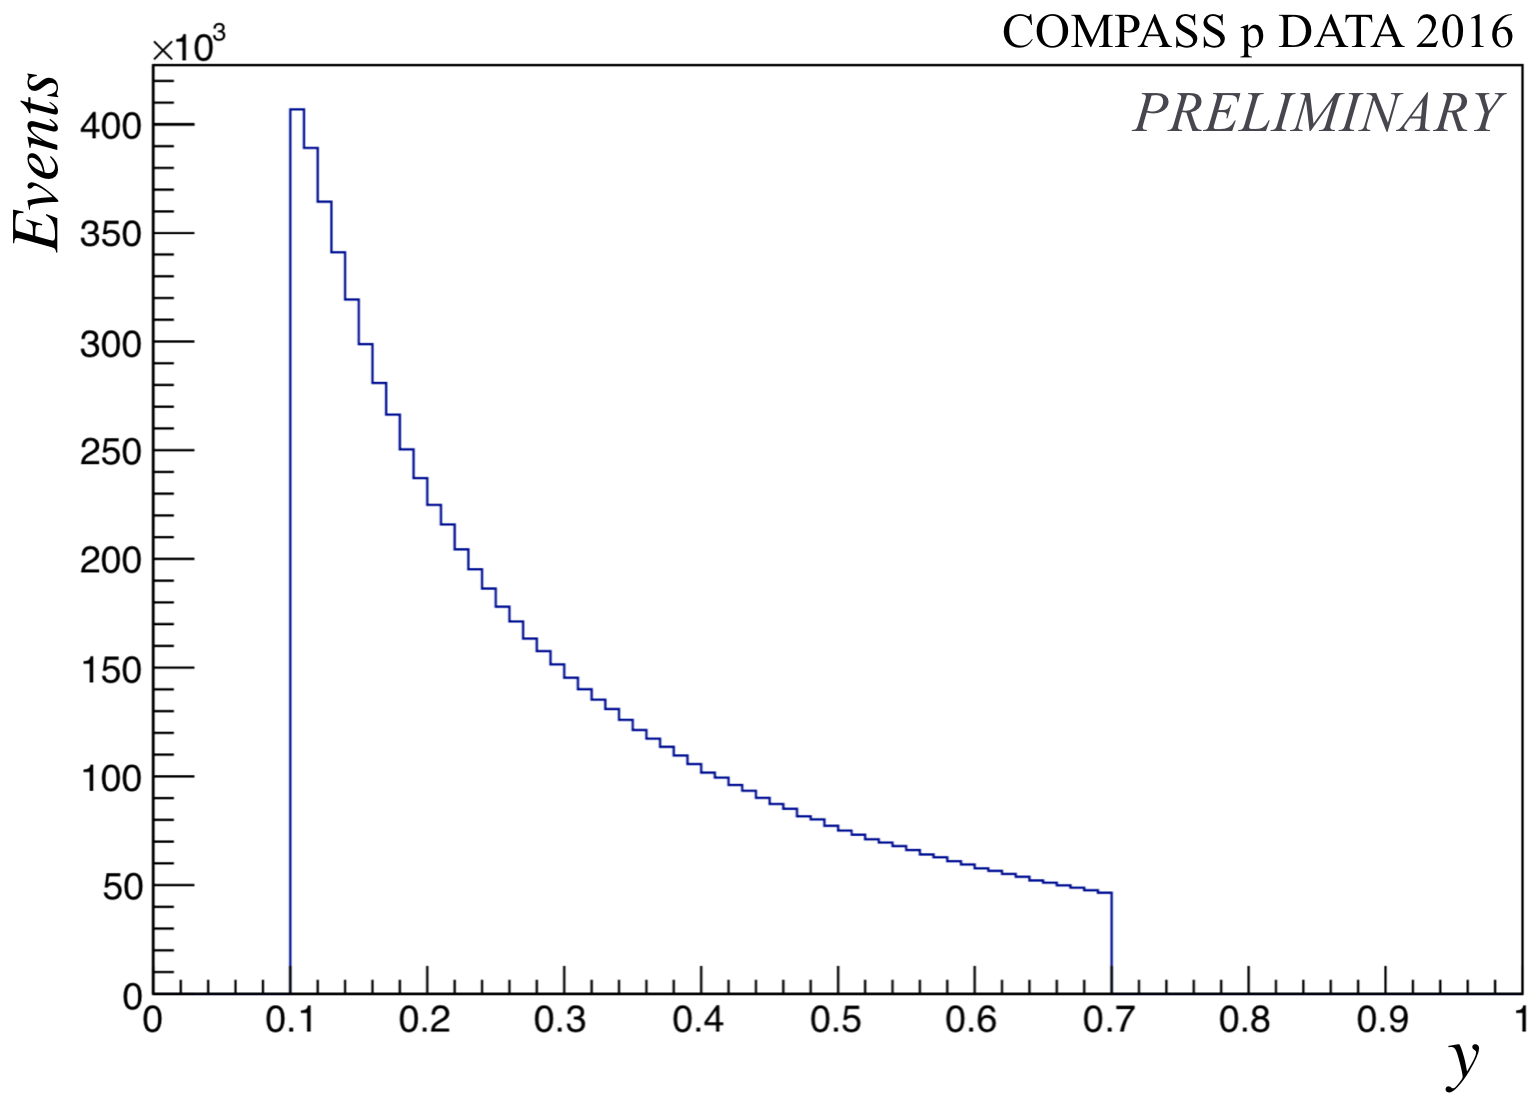
\includegraphics[scale=0.27]{./gfx/yDIS.png}} \\
  \subfloat[$x$-$Q^2$]{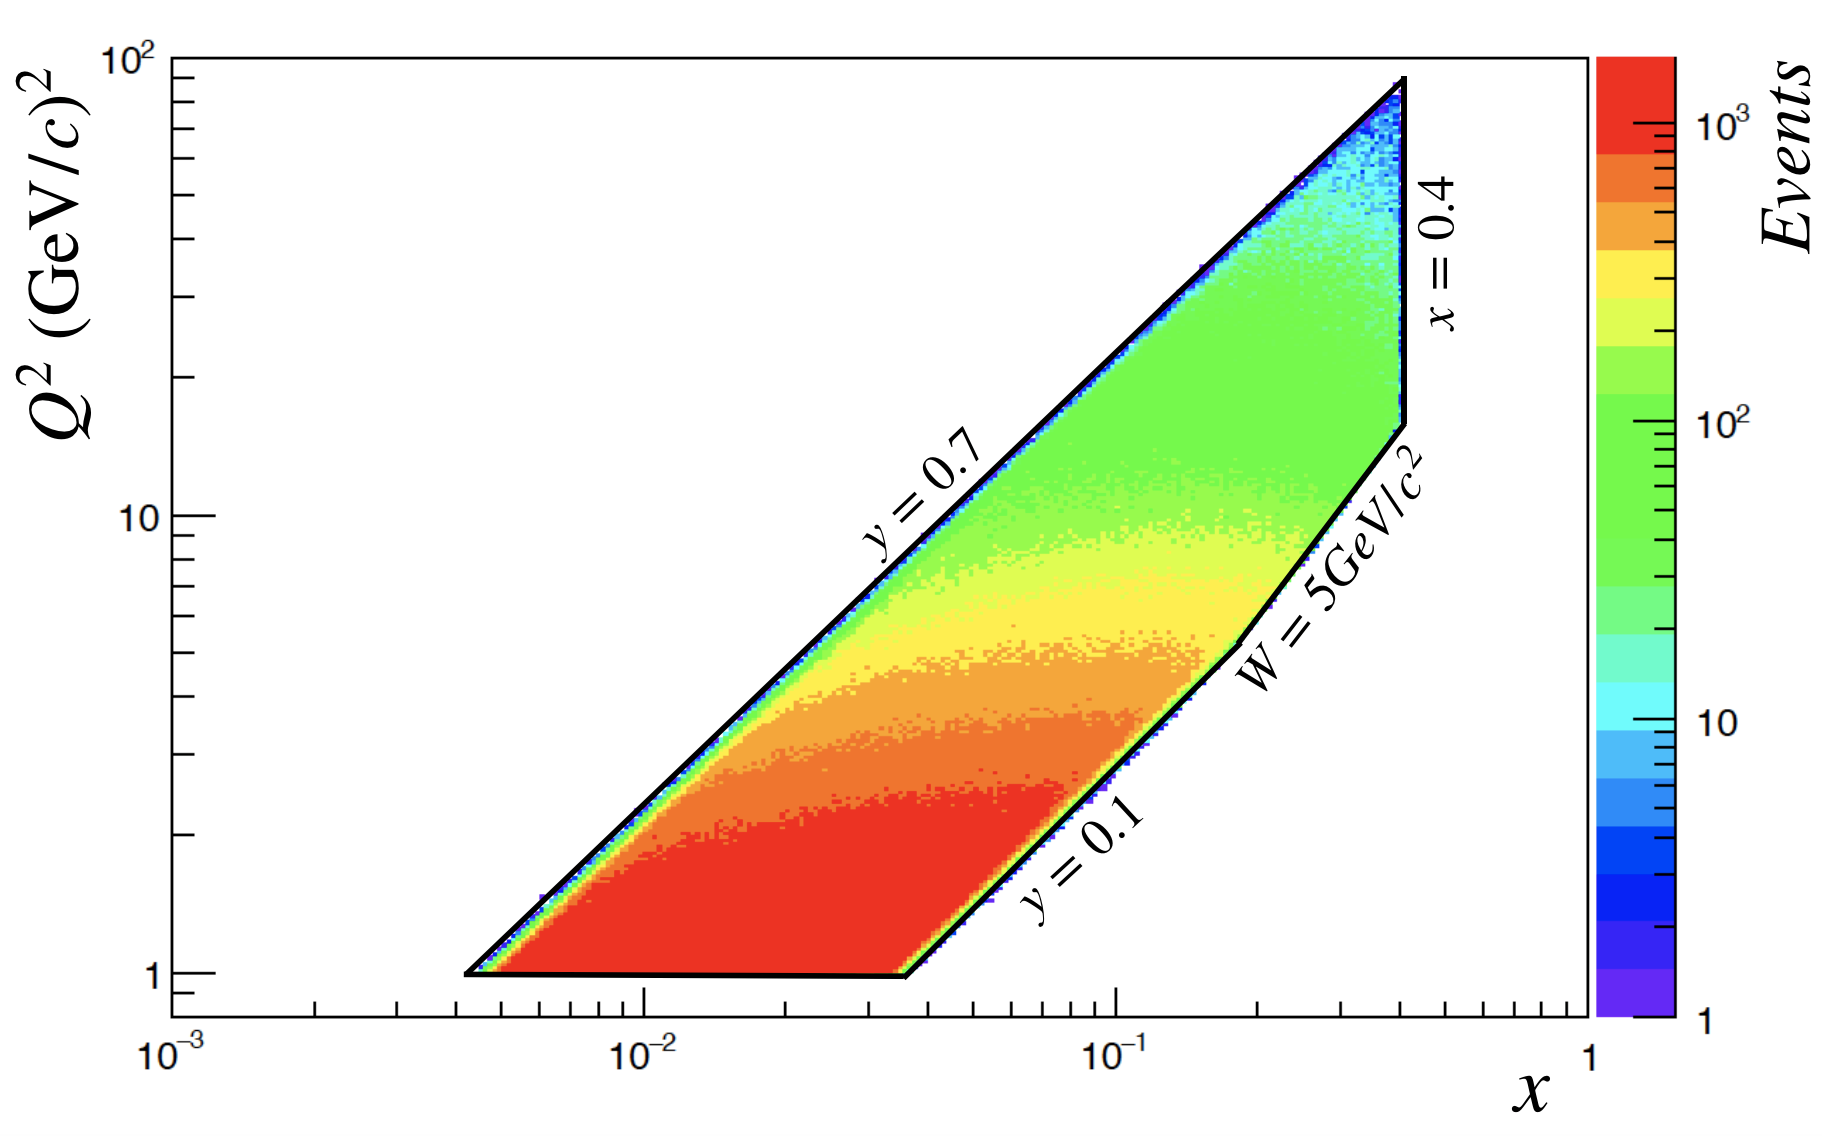
\includegraphics[scale=0.27]{./gfx/xQ2.png}}
  \subfloat[$x$-$y$]{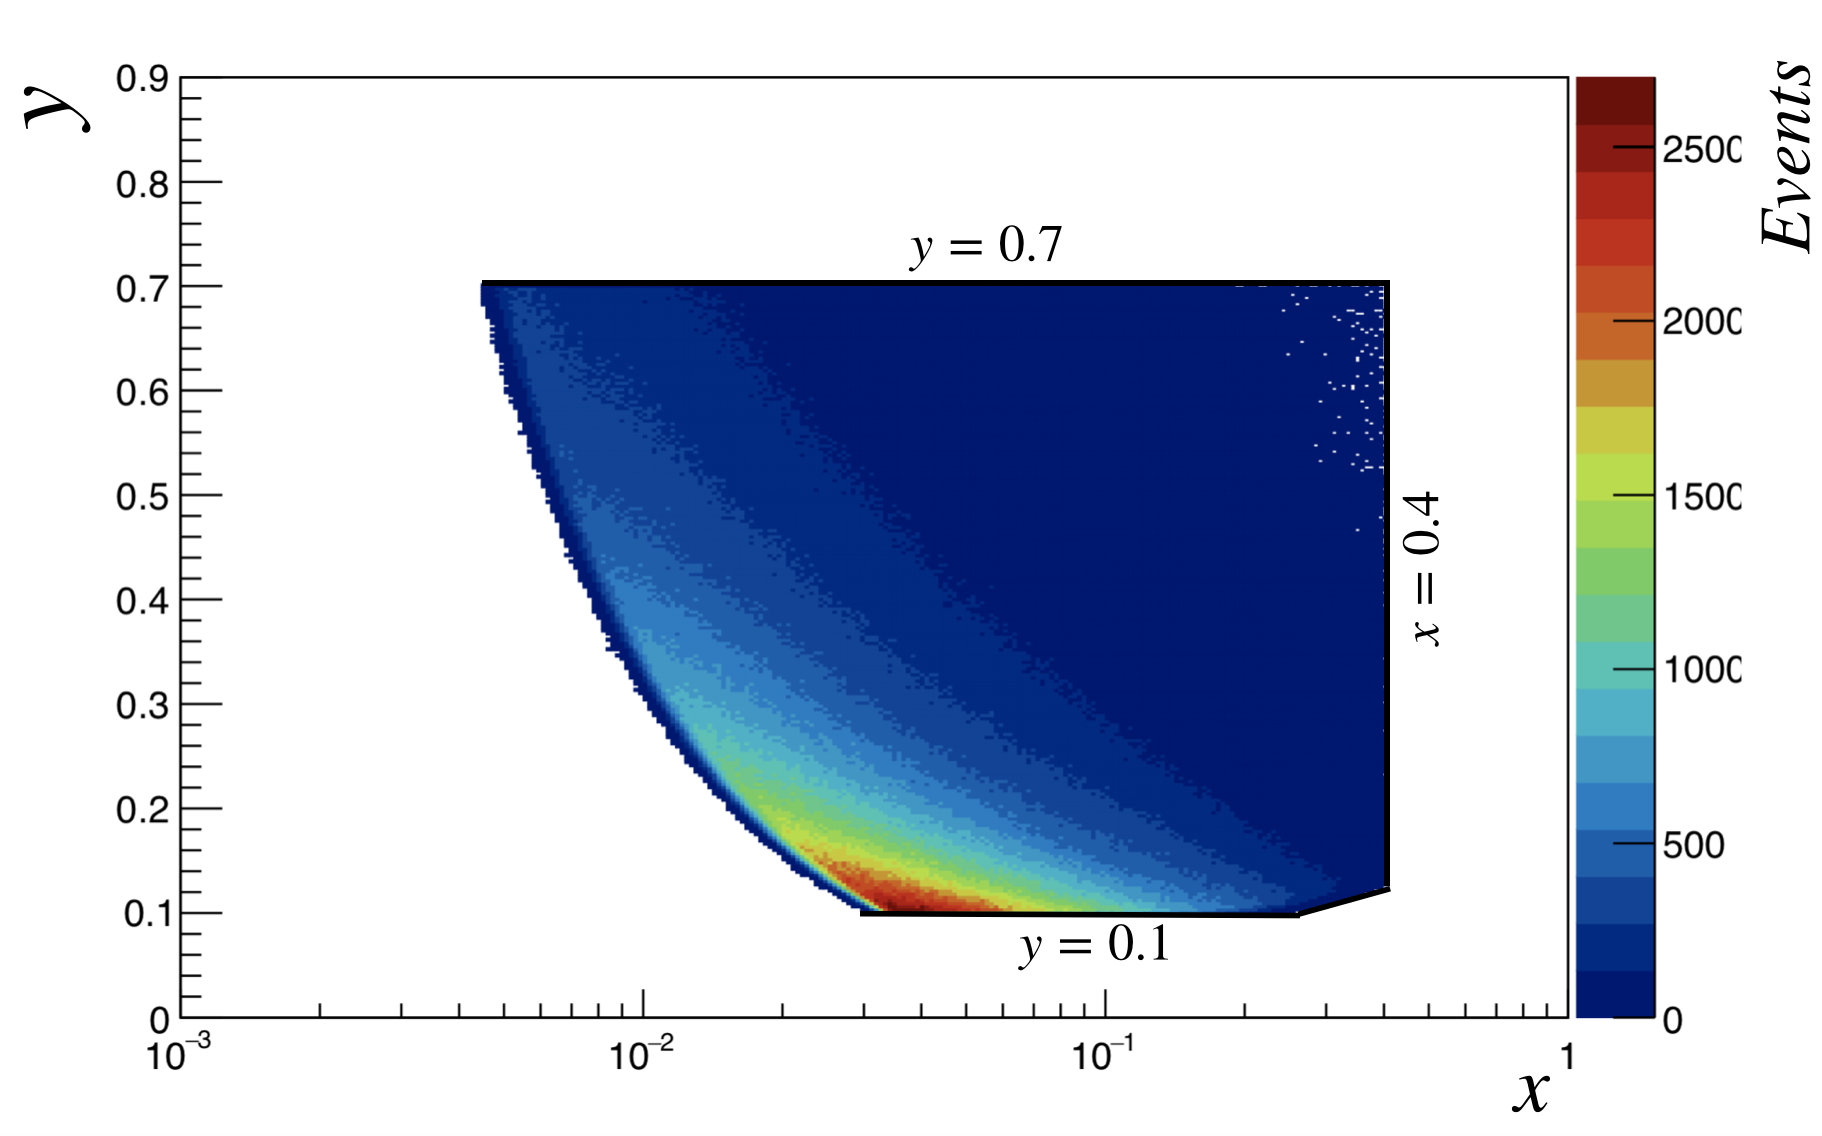
\includegraphics[scale=0.23]{./gfx/xy.png}}
	\caption{On the top panels, $Q^2$, $x$ and $y$ distributions. On the bottom, $Q^2$-$x$ and $x$-$y$ correlations. All distributions are for the final DIS sample.}
	\label{pic:DISdist}
\end{figure}

%------------------------------------------------

\section{Target cut evaluation} \label{sec:targetcut}

The 2m long $lH_2$ target in 2016 is long and not perfectly straight (slight 'banana shaped', Fig. \ref{pic:Target}), with a shape not easily reproducible in Monte-Carlo. The Monte-Carlo target is only a cylinder that was tilted by an angle extracted from the real data target. This angle corresponds to the angle between the upstream and downstream ends of the target. Of course due to its 'banana shape' in reality, the description of the target in Monte-Carlo is not reaching 100\% fidelity. After the radial cut on the real data target (1.9 cm radius and $y$ = 1.2 cm), the residual volume, which is the volume of the real data target remaining after intersection with the Monte-Carlo target, is of 0.5\% (Fig. \ref{pic:Target}). This brings a systematic error on the multiplicities that I wanted to avoid. To this end, I devised three different solutions :

\begin{figure}[!h]
	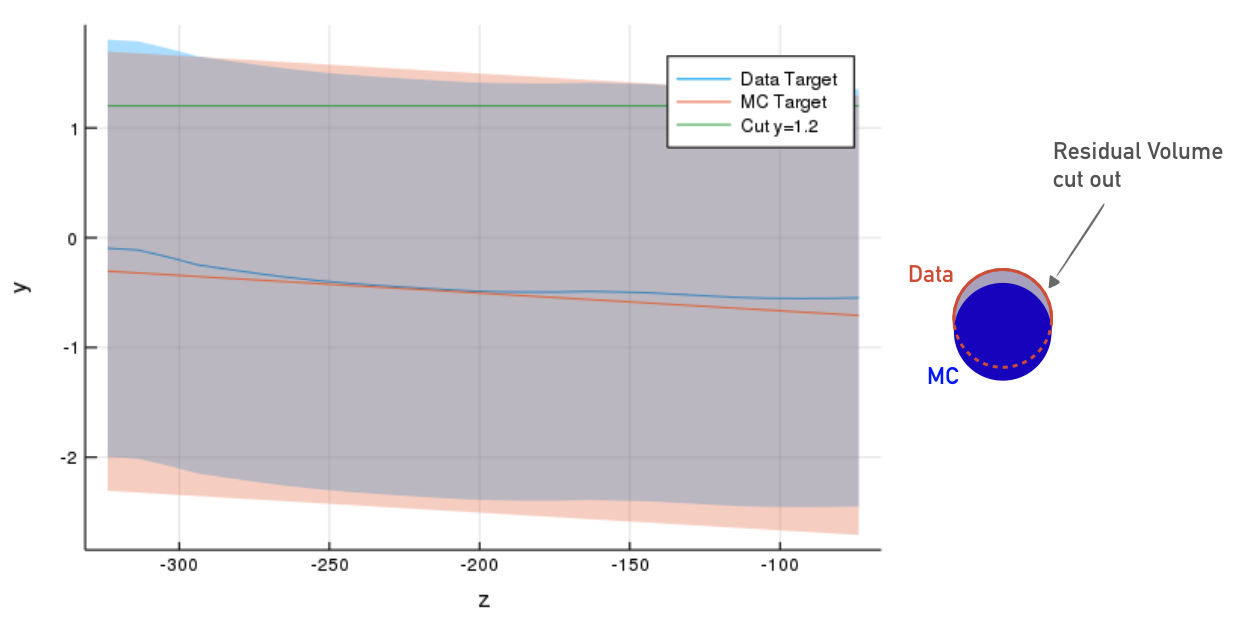
\includegraphics[scale=0.4]{./gfx/Targetcut.png}
	\caption{Left is a ($y$,$z$) view of the real data (blue) and the Monte-Carlo target (red), $z$ being the direction of propagation of the beam. The actual cut used in the analysis corresponds to the intersection of both real data target (red) and Monte-Carlo target (blue) volumes. Right is a sketch showing approximately how much we lose by doing such cut.}
	\label{pic:Target}
\end{figure}

\begin{enumerate}
  \item Cut more severely on the radius of the real data target (1.7 cm radial cut) to reduce the  residual volume to zero.
  \item Do a simultaneous cut on the real data target and on the Monte-Carlo target to only keep the intersection between the two volumes.
  \item Do a better description of the target in the Monte-Carlo by using several cylinder volumes and fuse them together to increase the fidelity of the Monte-Carlo target description with respect to the real data one.
\end{enumerate}

The last solution may be used in the future to maximise the efficiency of the analysis from a statistic point of view but it is heavy and time consuming for a marginal gain. We speak of a gain of at most 0.5\% with respect to the method we eventually chose, while one can argue that as the events we gain are on the edge of the target, thus might be cut out by subsquent cuts, the gain should even be less than this.
The first two solutions were in competition and had the same spirit : cut more in the data target to avoid any systematic bias between real data target and Monte-Carlo target. I chose the second one, a simultaneous cut on both targets, as it was the one that was discarding less target volume, thus maximising statistics. In Fig. \ref{pic:Target} you can see the volume that survives such cut.

%------------------------------------------------

\section{Downstream target vertex distribution}

We discovered when looking at vertex distribution for hadrons and comparing data with Monte-Carlo that there was a deficit of about 6\% of vertices in the downstream part of the target (between -100 and -70 cm, Fig. \ref{VertexDrop}). We saw this phenomenon both in data and Monte-Carlo however it was more stressed in data than in Monte-Carlo. After investigation, we discovered that, both in data and Monte-Carlo, there were a high number of hadrons that have their track not attached to the best primary vertex in a 2 mm-radius circle around the best primary vertex (Fig. \ref{CircleHadron}). This circle is only visible in the downstream part of the target while in the upstream part it is non-existant.

\begin{figure}[!h]
	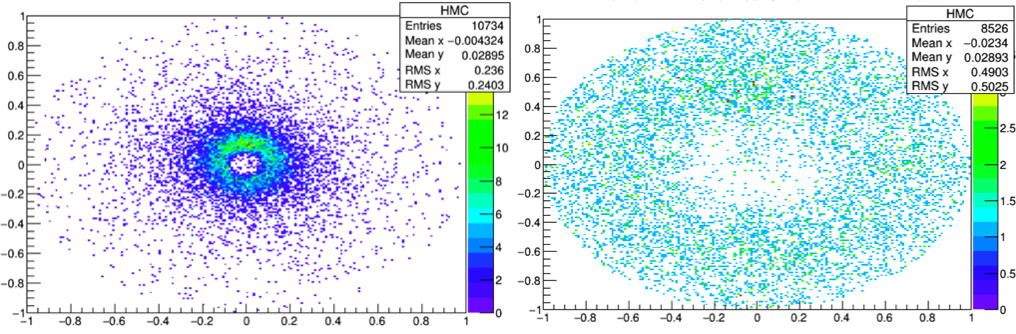
\includegraphics[scale=0.45]{./gfx/CircleHadron.png}
	\caption{Both plots are representing the relative distance to the best primary vertex of the extrapolated position of the unattached hadrons to the vertex position. On the left, the plot corresponds to the downstream part of the target and on the right, to the upstream part. The left plot shows an important amount of particles in a 2 mm-radius circle around the vertex while the right plot does not.}
	\label{CircleHadron}
\end{figure}

This issue might needs a thorough investigation of how the reconstruction is done in this case. However we found a rescue procedure to reattach these hadrons to the best primary vertex. All the hadrons in a circle of radius 2 mm around the best primary vertex are considered as if they were attached to it (considering they have a track ID and a momentum associated). With this procedure we were able to recover for the loss of hadron in the downstream part of the target (Fig. \ref{VertexDrop}).

\begin{figure}[!h]
	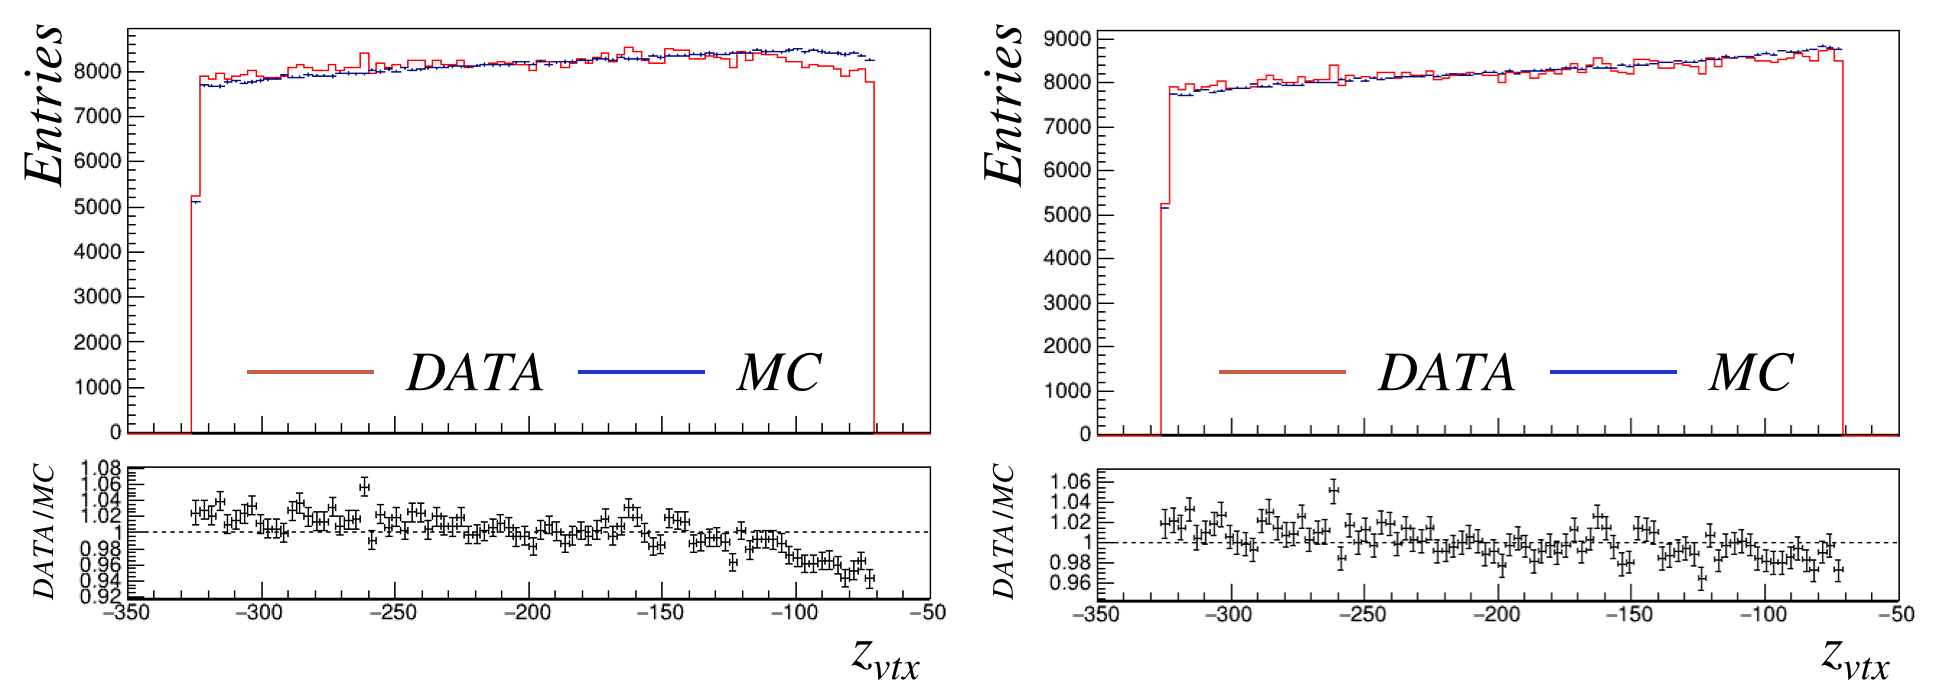
\includegraphics[scale=0.45]{./gfx/VertexDrop.png}
	\caption{One expects the vertex distribution for hadrons to increase with $z_{vtx}$ due to the apparatus acceptance. However in the left plot there is a drop both in data and Monte-Carlo of the number of vertices. In the right plot, after the rescue procedure, the drop has disappeared. The rescue procedure also reconciles data and Monte-Carlo.}
	\label{VertexDrop}
\end{figure}

One can fear that with such a procedure I attach back some hadrons that should not be attached. Here I bring two answers : a part of these 'bad' hadrons are hadrons reconstructed without associated momentum and are thus non-eligible to this rescue procedure. Another part are hadrons that will then be cut out by hadron cut, especially by the RICH entrance angle cut. A last part of these 'bad' hadrons will effectively be part of the hadron sample but I consider the 'bad' hadron fraction to be negligible compared to the 'good' hadrons fraction, thus no systematic uncertainty is applied concerning this rescue procedure. Again, this method is only temporary and this problem should be investigated more thoroughly in the future as it seems it is a long term problem within COMPASS reconstruction procedure.

%------------------------------------------------

\section{Hadron selection}

For the hadron selection ($\mu p \rightarrow \mu hX$), the following list of cuts is applied :
\begin{table}[!h]
  \centering
  \begin{tabular}{p{10cm} p{2cm} p{2cm}}
    \hline
    \hline
     Cut & \# of events after cut & Absolute \% of events after cut  \\
    \hline
    \hline
    Particle is not a scattered muon & 37.0 M & 100\% \\
    Maximum radiation length cumulated along all the trajectory < 15 radiation lengths & 28.3 M & 76.6\% \\
    $\chi^2$/ndf $<$ 10 for the hadron track & 27.9 M & 75.4\% \\
    Z coordinate of the first measured hit < 350 cm & 27.9 M & 75.3\% \\
    Z coordinate of the last measured hit > 350 cm & 19.1 M & 51.5\% \\
    $0.01 < \theta_{RICH} < 0.12$ (at RICH entrance) & 12.6 M & 34.1\% \\
    $x^2_{RICH} + y^2_{RICH} > 25$ cm$^2$ (rejection of RICH pipe) & 12.5 M & 33.7\% \\
    $12 < p_h < 40$ GeV/$c$ & 3.37 M & 9.11\% \\
    $0.2 < z < 0.85$ & 2.67 M & 7.21\% \\
    \hline
    \hline
  \end{tabular}
\end{table}

%----------------------------------------------------------------------------------------

\section{Particle Identification with RICH detector}

The $\pi$ and $K$ particle identification (PID) is performed by the RICH detector.

The method used for the RICH particle identification is described in Chapter. \ref{ch:PID}. The idea is the following : when a particle is detected, six likelihood (LH) functions are calculated ($\pi$, $K$, $p$, $e$, $\mu$ and the background) and are then compared to make the particle identification. The evaluation is done separately for pions, kaons and protons. The largest value corresponds to the maximal probability. The method is improved by looking further to $LH(2^{nd})$ which is the second highest value of the four compared likelihood values ($\pi$, $K$, $p$ and the background). The electron and muon likelihoods are not considered in the assignment of $LH(2^{nd})$ as in the chosen momentum range (12 to 40 GeV/c) the RICH detector can not be used to efficiently distinguish electrons from $\pi$.

All $\pi$, $K$ and $p$ probabilities are needed for the unfolding. The likelihood cuts were optimized as follows :

\begin{enumerate}
  \item Pion selection
  \begin{itemize}
    \item $LH(\pi) > 0$
    \item $LH(\pi) > LH(K)$, $LH(p)$ and $LH(bg)$.
    \item $\frac{LH(\pi)}{LH(2^{nd})}>1.02$
    \item $\frac{LH(\pi)}{LH(bg)}>2.02$
  \end{itemize}
  \item Kaon selection
  \begin{itemize}
    \item $LH(K) > 0$
    \item $LH(K) > LH(\pi)$, $LH(p)$ and $LH(bg)$.
    \item $\frac{LH(K)}{LH(2^{nd})}>1.08$
    \item $\frac{LH(K)}{LH(bg)}>2.08$
  \end{itemize}
  \item Proton selection
  Three cases are considered depending on the momentum $p_{h}$ of the particle and are distinguished by the kaon threshold ($\simeq 8.9$ GeV/c) and proton threshold ($\simeq 17.95$ GeV/c) :
  \begin{enumerate}[(a)]
    \item Kaon threshold $< p_{h} \leq$ proton threshold - 5 GeV/c
	  \begin{center}
		  \begin{tabular}{c|c}
		    \hline
		     $p$ & $\bar{p}$ \\
		    \hline
				\multicolumn{2}{c}{Not to be a $\pi$ or $K$} \\
		    $\frac{LH(\pi)}{LH(bg)} < 2.2$ & $\frac{LH(\pi)}{LH(bg)} < 2.1$ \\
		    $\frac{LH(K)}{LH(bg)} < 2.9$ & $\frac{LH(K)}{LH(bg)} < 2.8$ \\
		    \hline
				\multicolumn{2}{c}{or all $LH$ = 0} \\
				\hline
		  \end{tabular}
		\end{center}
    \item $p_{h} >$ proton threshold + 5 GeV/c
    \begin{itemize}
      \item $LH(p) > 0$
      \item $LH(p) > LH(\pi)$, $LH(K)$ and $LH(bg)$.
      \item $\frac{LH(p)}{LH(2^{nd})}>1$
    \end{itemize}
    \item Proton threshold - 5 GeV/c $< p_{h} <$ proton threshold + 5 GeV/c
    \begin{itemize}
      \item Using (a) and (b) simultaneously.
    \end{itemize}
  \end{enumerate}
\end{enumerate}

%----------------------------------------------------------------------------------------

\section{RICH unfolding based on efficiency matrices}

The performance of the RICH is not perfect : neither in terms of efficiency nor in terms
of purity.

The unfolding procedure is needed to correct the yield of identified hadrons for this imperfection.
In order to perform this correction, the RICH actual performance is evaluated from real data. The result of
this evaluation is presented through RICH performance matrices, $M_{RICH}$, binned in momentum
and angle :

\begin{itemize}
  \item $p_h$ \{12,13,15,17,19,22,25,27,30,35,40\} GeV/c
  \item $\theta$ \{0.01,0.04,0.12\} rad
\end{itemize}

The 3-by-3 matrices $M_{RICH}$ give a relation between the vector of counts for true hadron $T_h$ and the vector for identified hadron $I_h$ :

\begin{equation}
\begin{bmatrix}
I_{\pi} \\
I_K \\
I_p
\end{bmatrix}
=
\begin{bmatrix}
\epsilon(\pi \rightarrow \pi) & \epsilon(K \rightarrow \pi) & \epsilon(p \rightarrow \pi)\\
\epsilon(\pi \rightarrow K) & \epsilon(K \rightarrow K) & \epsilon(p \rightarrow K) \\
\epsilon(\pi \rightarrow p) & \epsilon(K \rightarrow p) & \epsilon(p \rightarrow p)
\end{bmatrix}
\begin{bmatrix}
T_{\pi} \\
T_K \\
T_p
\end{bmatrix}
\end{equation}

The coefficients of the $M_{RICH}$, $\epsilon(t \rightarrow i)$, are the probabilities that a true hadron
$t$ is identified as a hadron of type $i$. These probabilities have been determined as described in Chapter. \ref{ch:PID}.

The number of true hadrons are obtained by inverting the performance matrices (Eq. \ref{richmat}) :

\begin{equation}
  \overrightarrow{T_h} = M^{-1}_{RICH}\overrightarrow{I_h}
	\label{richmat}
\end{equation}

\begin{table}[!h]
  \caption{\label{HadNum} Number of identified pions, kaons, and protons for the 5 periods before and after unfolding.}
  \centering
  \begin{tabular}{lcccccc}
    \hline
     & $\pi^+$ & $\pi^-$ & $K^+$ & $K^-$ & $p$ & $\bar{p}$ \\
    \hline
    Identified & 953970 & 789480 & 253045 & 153440 & 131066 & 60705 \\
    Unfolded & 976213 & 814685 & 255132 & 150775 & 124221 & 52014 \\
    \hline
  \end{tabular}
\end{table}

%----------------------------------------------------------------------------------------

\section{Kinematic binning}

The raw multiplicities are evaluated in bins of the Bjorken variable $x$, the muon energy fraction carried by the virtual photon $y$ and the virtual photon energy fraction carried by final state hadron $z$. They are calculated with the following formula :

\begin{equation}
  \frac{dM^h(x,y,z)}{dz}=\frac{1}{N^{DIS}_{Events}(x,y)}\frac{dN^{DIS}_{h}(x,y,z)}{dz}
\end{equation}

where $N^{DIS}_{Events}$ is the number of DIS events and $N^{DIS}_{h}$ is the number of
hadrons after RICH unfolding. As in practise, the multiplicities are measured in bins of
x (9 bins), y (5 bins) and z (12 bins), the calculated multiplicities can be expressed as :

\begin{equation}
  M^h_{raw}(x,y,z) = \frac{N^{DIS}_{h}(x,y,z)/\delta z}{N^{DIS}_{Events}}
\end{equation}

where $\delta z$ is the width of the z bin. For the multiplicities extraction, the binning in
$x$, $y$ and $z$ is the following :

\begin{table}[!h]
  \centering
  \caption{Multidimensional binning for the multiplicity extraction}
  \label{tab:kinbinning}
  \begin{tabular}{ll}
    \hline
    \hline
    Variable & Binning \\
    \hline
    \hline
    $x$ & \{0.004,0.01,0.02,0.03,0.04,0.06,0.1,0.14,0.18,0.4\} \\
    $y$ & \{0.1,0.15,0.2,0.3,0.5,0.7\} \\
    $z$ & \{0.2,0.25,0.3,0.35,0.4,0.45,0.5,0.55,0.6,0.65,0.7,0.75,0.85\} \\
    \hline
    \hline
  \end{tabular}
\end{table}

%----------------------------------------------------------------------------------------

\section{Statistical error propagation}

The statistical error propagation used in the multiplicity calculation will be explained in the following. Looping through DIS events, the squared error is :

\begin{equation}
		E^2_{DIS} = 1
\end{equation}

Looping through unidentified hadrons, the squared error is :

\begin{equation}
		E^2_{Had} = 1
\end{equation}

For identified hadrons, the squared error includes the RICH statistical error :

\begin{equation}
		E^2_{Had} = E^2_{RICH}
\end{equation}

where

\begin{equation}
		E^2_{RICH}[0<h<3] = cov(M^{-1}_{hr},M^{-1}_{hr})+(M^{-1}_{hr})^2
\end{equation}

with $M_{hr}$ the element of the RICH unfolding matrix for hadron $h$ from RICH identified hadron $r$ and

\begin{equation}
		cov(M^{-1}_{hr},M^{-1}_{hr}) = \sum_{0<i,j,k,l<3} M^{-1}_{hi}M^{-1}_{jr}M^{-1}_{hk}M^{-1}_{lr}cov(M_{ij},M_{kl})
\end{equation}

For the raw multiplicities the error takes into account the correlation between hadrons and DIS events :

\begin{equation}
		E^2_{raw} = \Bigg[\frac{E^2_{Had}}{N^2_{DIS}} - \bigg( \frac{N^2_{Had}}{N^2_{DIS}} \bigg)^2 E^2_{DIS} \Bigg]/z^2_{width}
\end{equation}

\section{Results for raw multiplicities ($h^{\pm}$, $\pi^{\pm}$, $K^{\pm}$ and $p/\bar{p}$)}

The raw multiplicity results shown in this section are without any correction except the RICH unfolding correction for identified hadrons. The unidentified hadron, the pion, the kaon and the proton multiplicities are displayed as a function of $z$ in bins of $x$ and staggered vertically with $y$ in Figs. \ref{pic:rawhp} to \ref{pic:rawpm}. The charged hadron multiplicities strongly depends on $z$ as expected with a small dependence with $x$ also.

The $h^+$/$h^-$, $\pi^+$/$\pi^-$ and $p/\bar{p}$ raw multiplicities are very similar but with a small asymmetry at high $x$, explained by the fact that at high $x$, the valence region, the $u$ quark is dominant. For kaons, $M_{raw}^{K^+} > M_{raw}^{K^-}$ as $K^-$ ($\bar{u}s$) can only be produced by sea quarks.

In total each charged hadron multiplicities are accounting for more than 300 data points.

\begin{figure}[!h]
	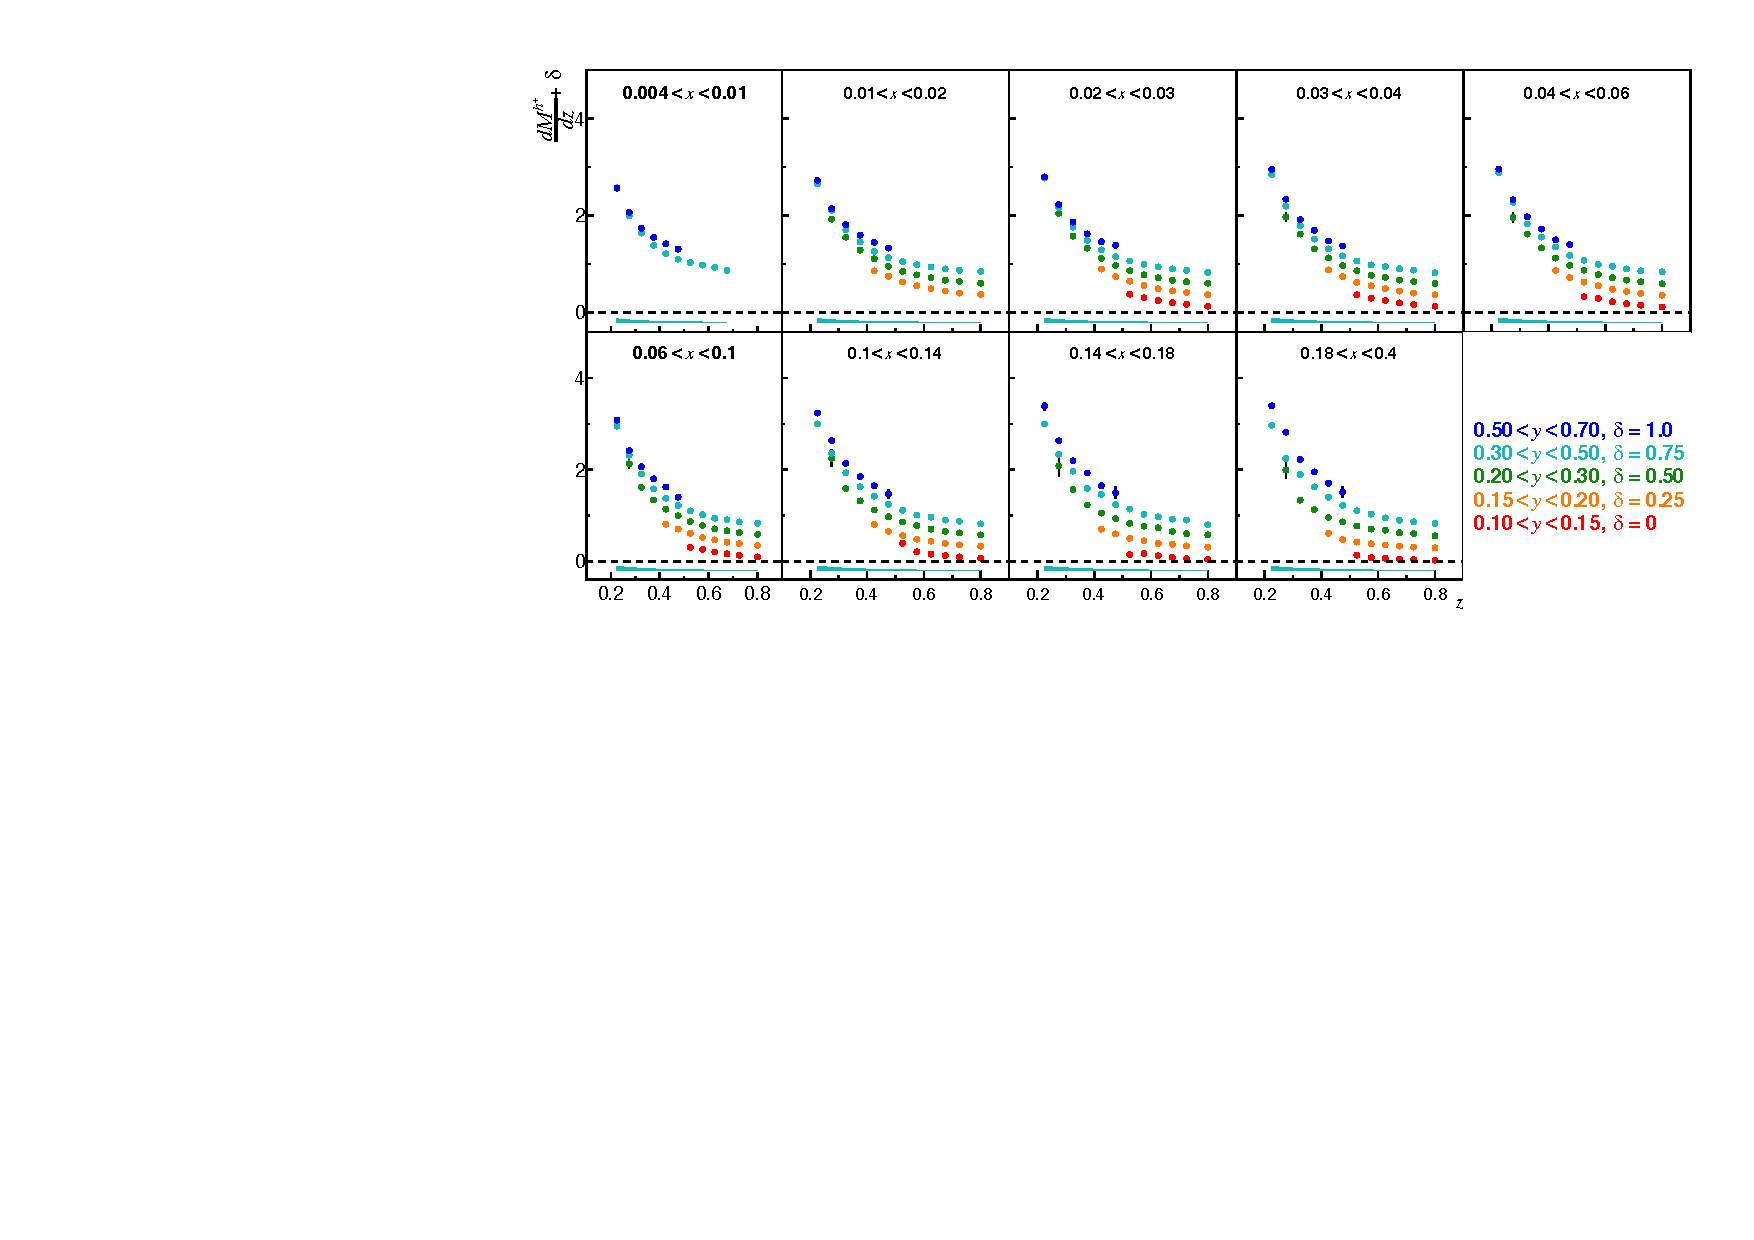
\includegraphics[scale=0.85]{./gfx/rawhp.pdf}
	\caption{Unidentified positive hadron raw multiplicities as a function of $z$ in bins of $x$ and scattered vertically with $y$. Statistical error is shown but is small in most of the bins.}
	\label{pic:rawhp}
\end{figure}

\newpage

\begin{figure}[!h]
  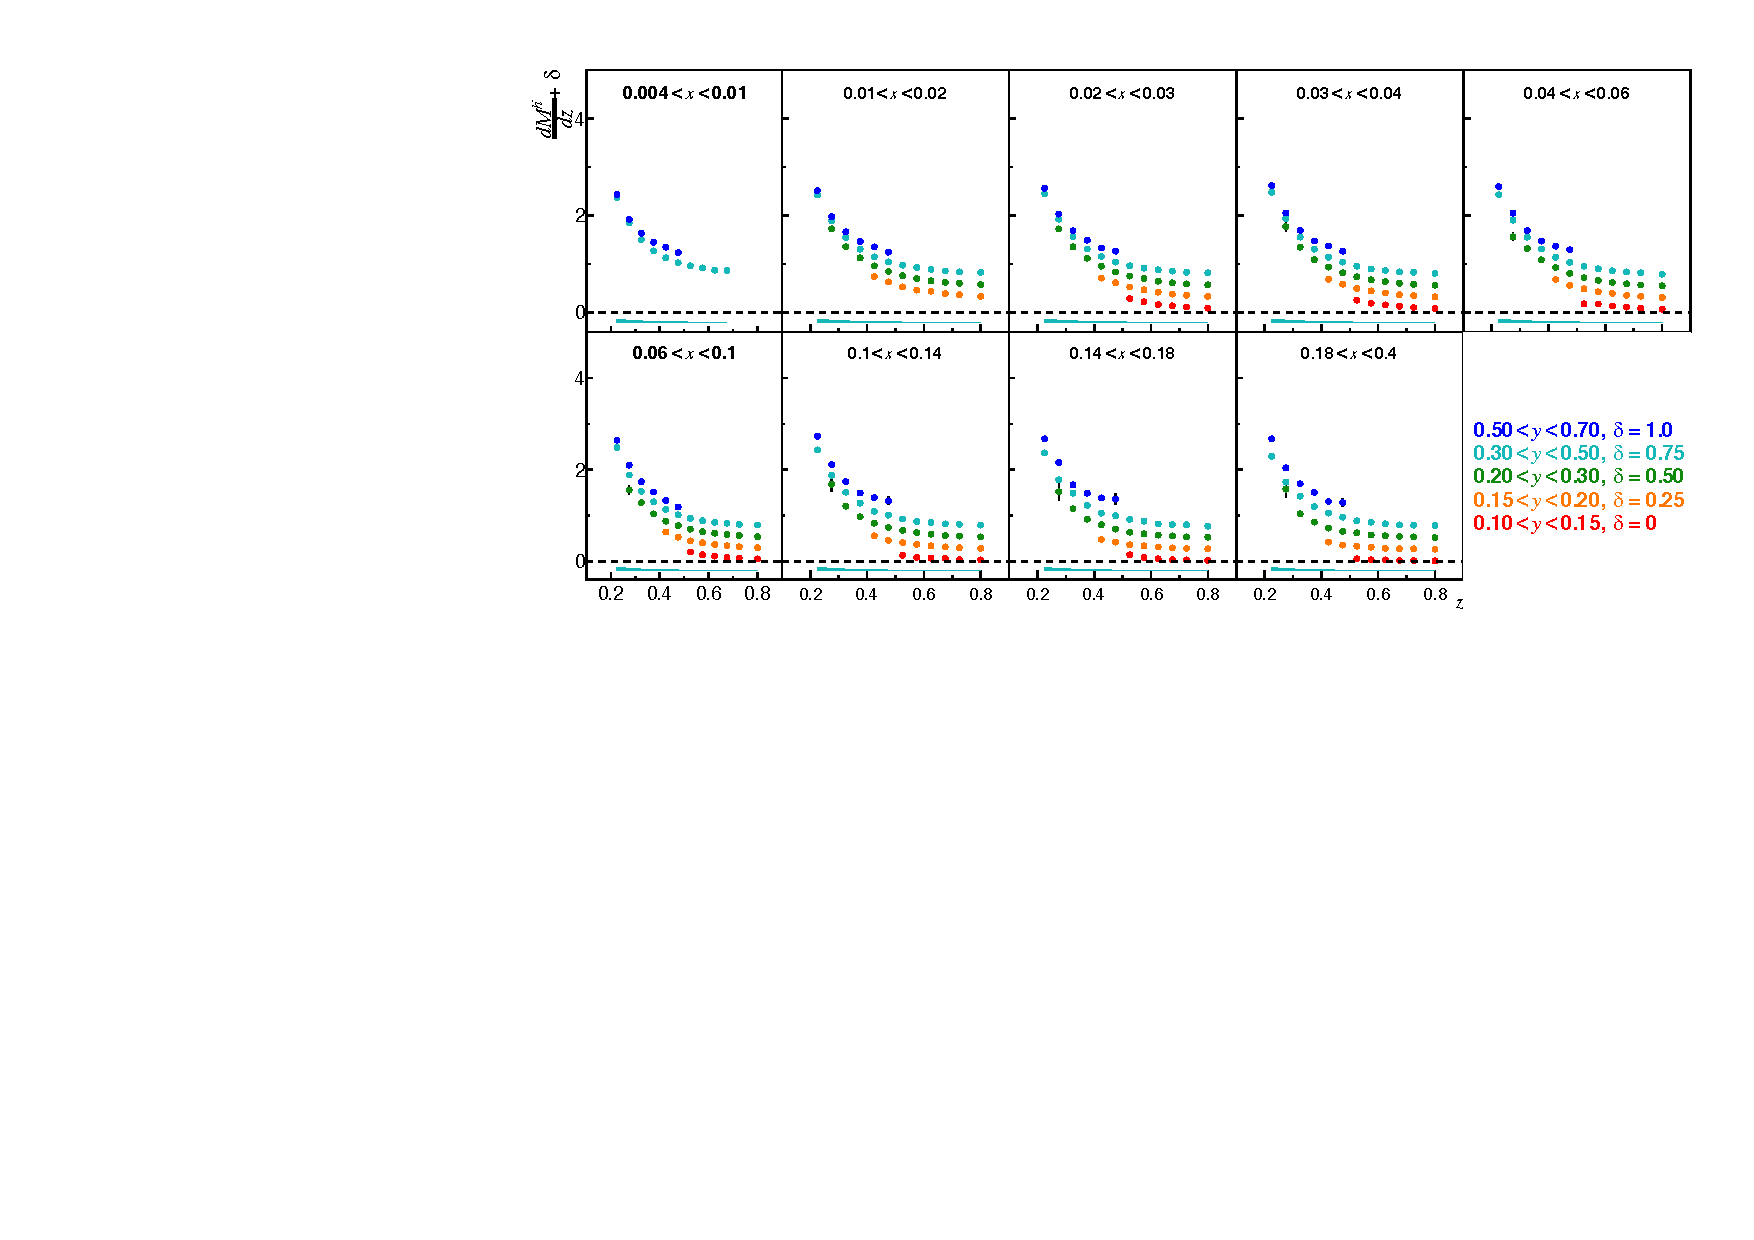
\includegraphics[scale=0.85]{./gfx/rawhm.pdf}
  \caption{Same as Fig. \ref{pic:rawhp} but for unidentified negative hadrons.}
  \label{pic:rawhm}
\end{figure}

\begin{figure}[!h]
  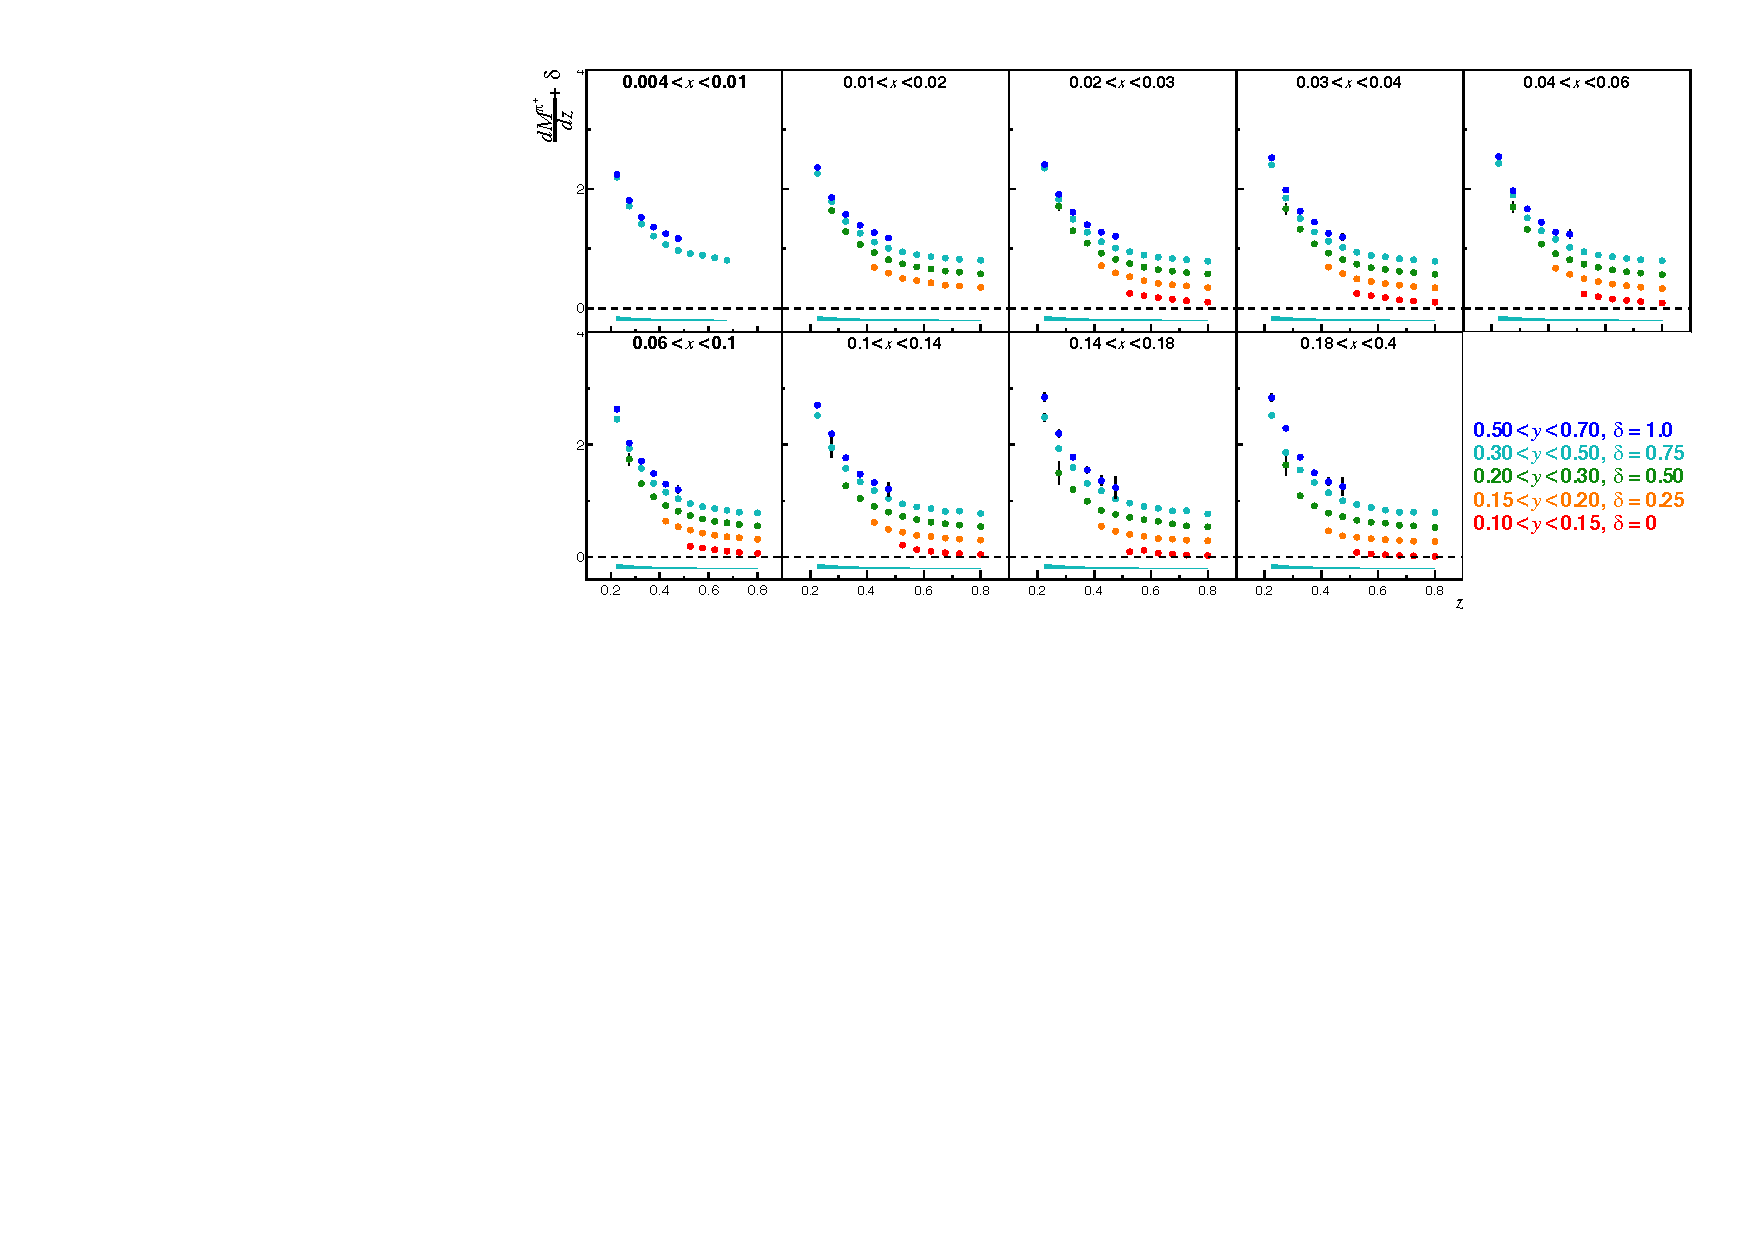
\includegraphics[scale=0.85]{./gfx/rawpip.pdf}
  \caption{Same as Fig. \ref{pic:rawhp} but for positive pions.}
  \label{pic:rawpip}
\end{figure}

\newpage

\begin{figure}[!h]
  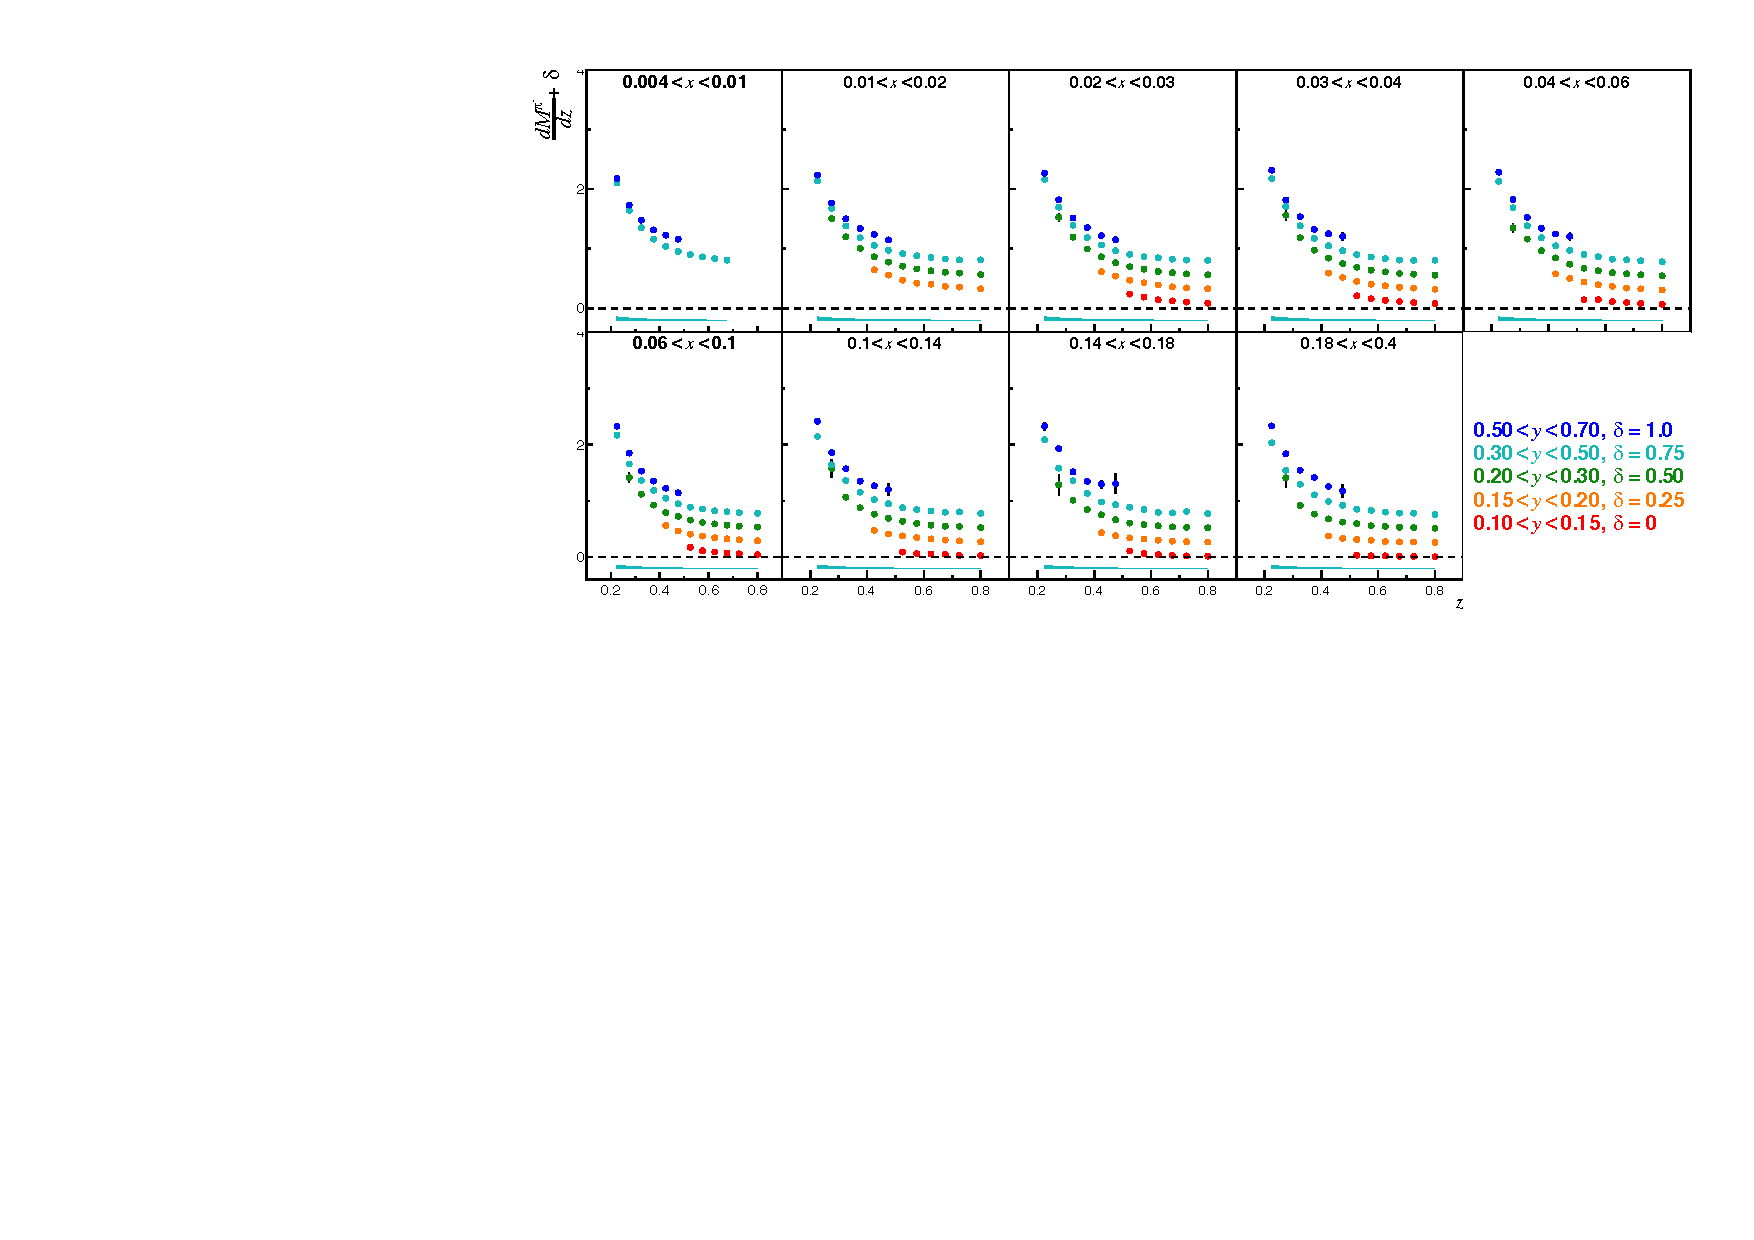
\includegraphics[scale=0.85]{./gfx/rawpim.pdf}
  \caption{Same as Fig. \ref{pic:rawhp} but for negative pions.}
  \label{pic:rawpim}
\end{figure}

\begin{figure}[!h]
  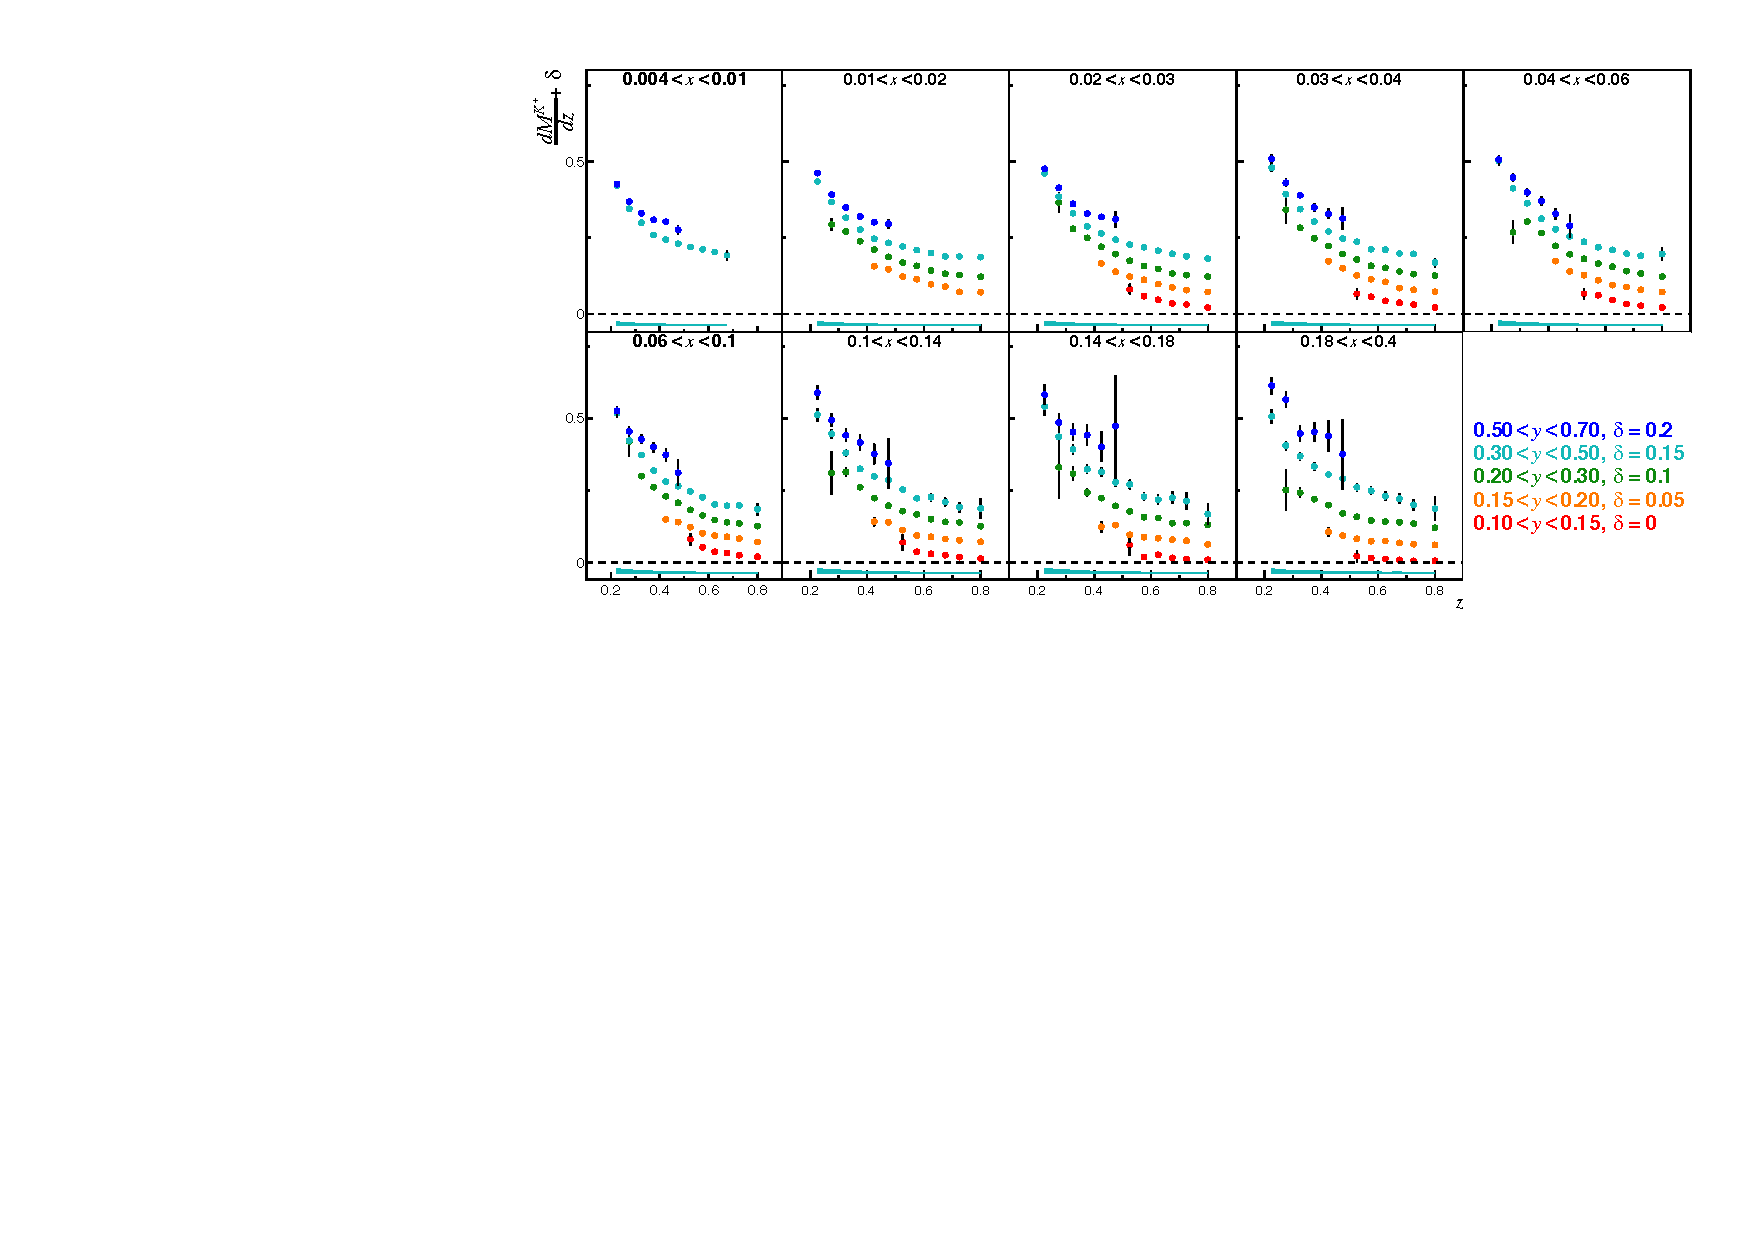
\includegraphics[scale=0.85]{./gfx/rawkp.pdf}
  \caption{Same as Fig. \ref{pic:rawhp} but for positive kaons.}
  \label{pic:rawkp}
\end{figure}

\newpage

\begin{figure}[!h]
  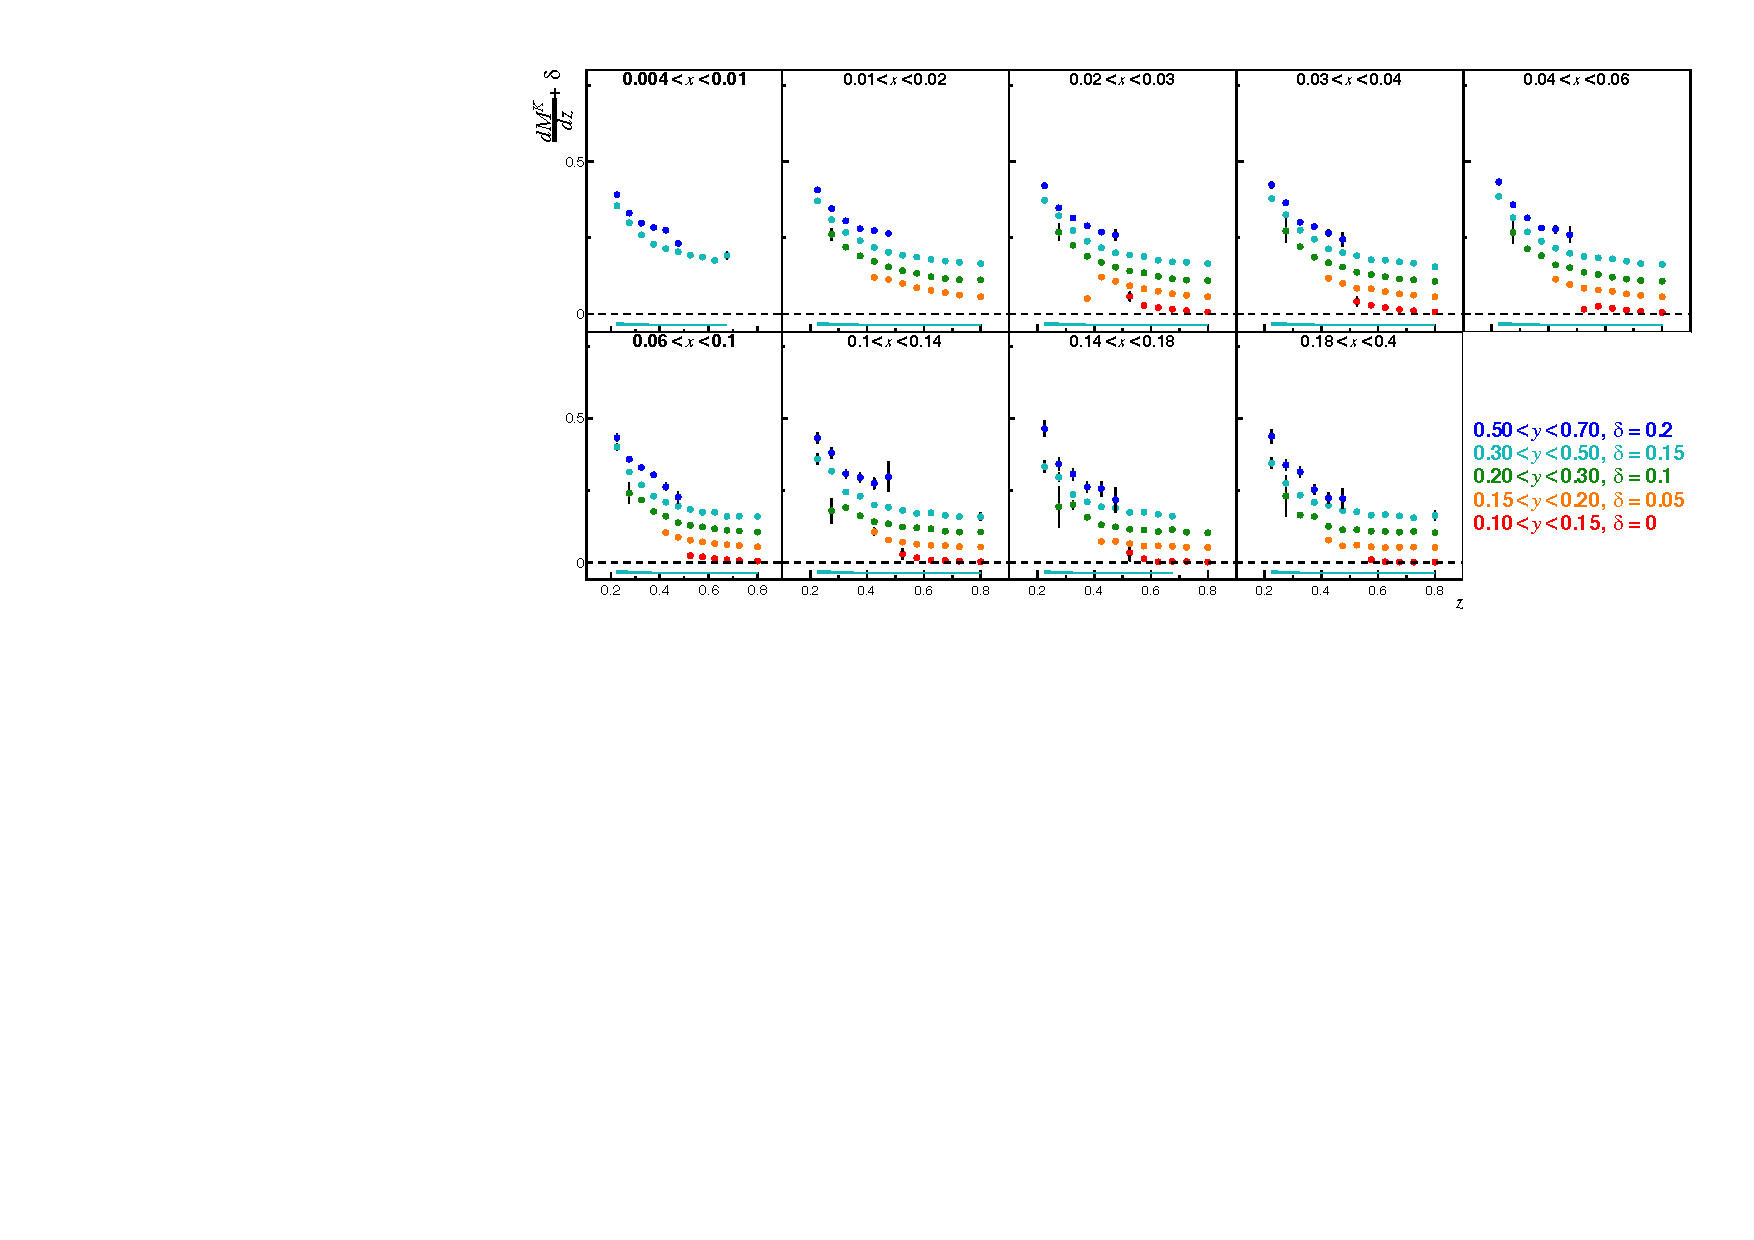
\includegraphics[scale=0.85]{./gfx/rawkm.pdf}
  \caption{Same as Fig. \ref{pic:rawhp} but for negative pions.}
  \label{pic:rawkm}
\end{figure}

\begin{figure}[!h]
  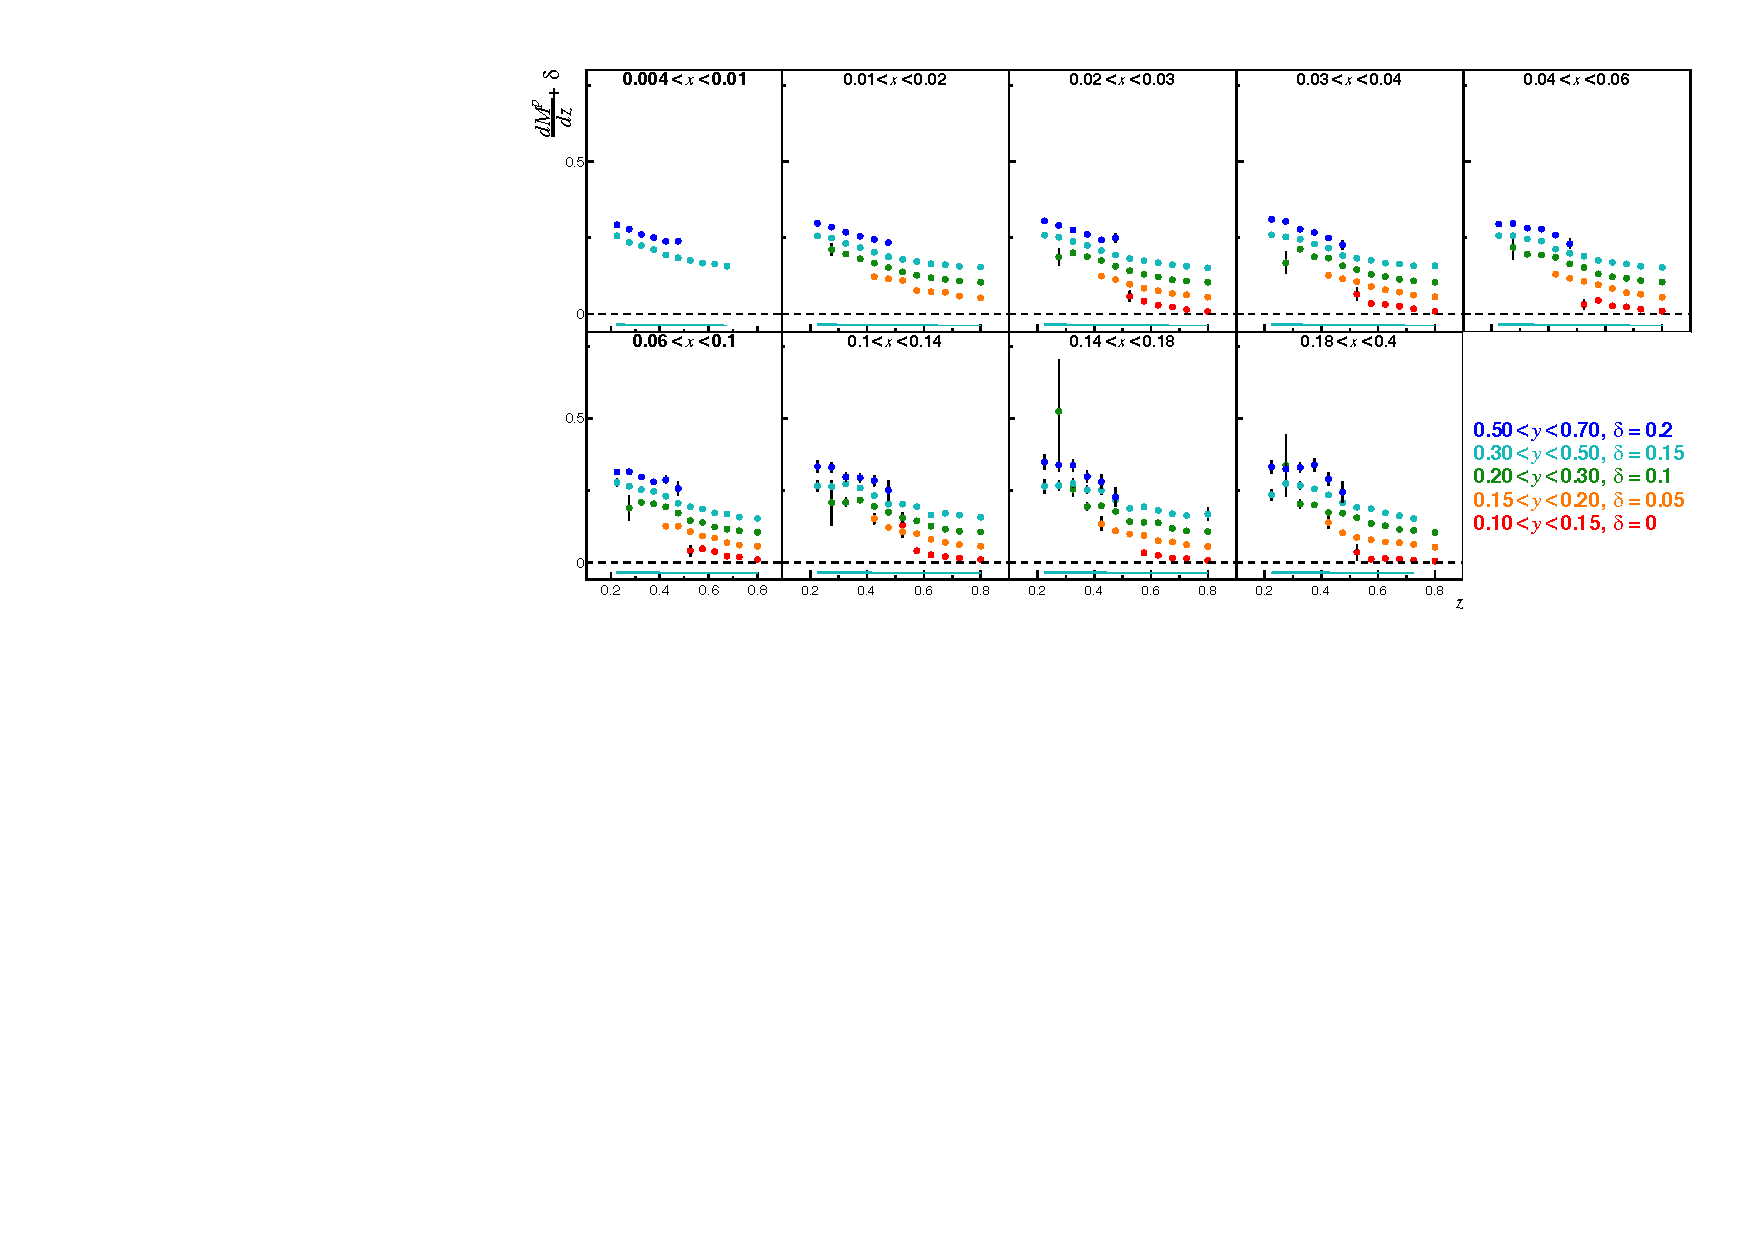
\includegraphics[scale=0.85]{./gfx/rawpp.pdf}
  \caption{Same as Fig. \ref{pic:rawhp} but for protons.}
  \label{pic:rawpp}
\end{figure}

\newpage

\begin{figure}[!h]
  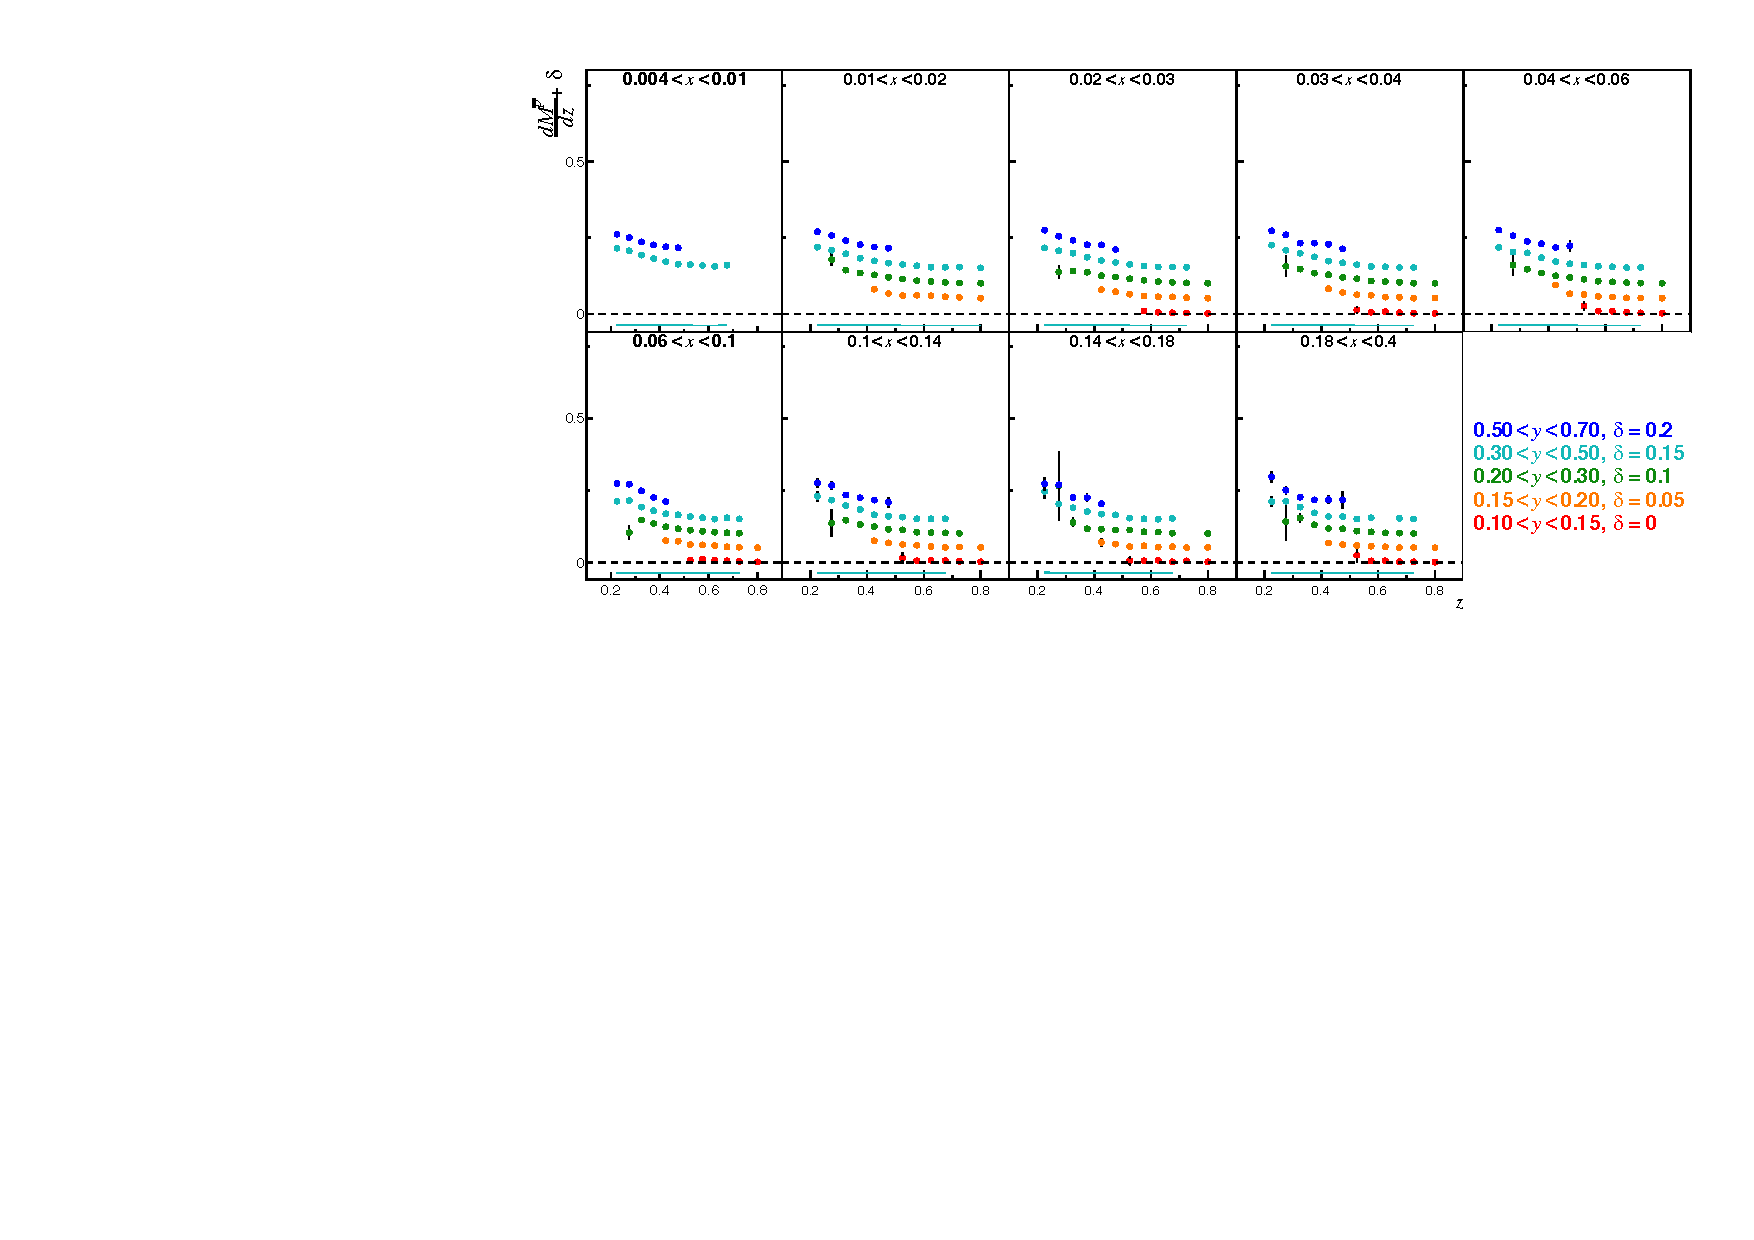
\includegraphics[scale=0.85]{./gfx/rawpm.pdf}
  \caption{Same as Fig. \ref{pic:rawhp} but for antiprotons.}
  \label{pic:rawpm}
\end{figure}

\section{Summary}

From muon deep inelastic scattering on a pure proton target (lH$_2$) from the 2016 COMPASS data, raw multiplicities for unidentified hadrons, pions, kaons and protons were extracted in a three dimensional ($x$,$y$,$z$) binning. The data cover a wide kinematic domain defined by $Q^2$ $>$ 1 (GeV/$c$)$^2$, $y$ $\in$ [0.1,0.7], $x$ $\in$ [0.004,0.4], $W$ $\in$ [5,17] GeV and $z$ $\in$ [0.2,0.85]. The hadron momentum is taken in the range [12,40] GeV/$c$.

The raw multiplicities for identified hadrons are corrected by the RICH identification and misidentification efficiencies. The dominant uncertainty, before the application of corrector factors, is the statistical error ($\sigma$/$M^h_{raw}$ < 1\%).
